% Conditionals
\newif\ifdoubleblind
\doubleblindtrue    % comment to get non-anonymized version
\newif\iflackofspace
\lackofspacetrue    % comment to get long version
\newif\ifrelatedworktable
% \relatedworktabletrue   % comment for textual description of search spaces in related work

%%
%% This is file `sample-sigconf.tex',
%% generated with the docstrip utility.
%%
%% The original source files were:
%%
%% samples.dtx  (with options: `all,proceedings,bibtex,sigconf')
%% 
%% IMPORTANT NOTICE:
%% 
%% For the copyright see the source file.
%% 
%% Any modified versions of this file must be renamed
%% with new filenames distinct from sample-sigconf.tex.
%% 
%% For distribution of the original source see the term`s
%% for copying and modification in the file samples.dtx.
%% 
%% This generated file may be distributed as long as the
%% original source files, as listed above, are part of the
%% same distribution. (The sources need not necessarily be
%% in the same archive or directory.)
%%
%%
%% Commands for TeXCount
%TC:macro \cite [option:text,text]
%TC:macro \citep [option:text,text]
%TC:macro \citet [option:text,text]
%TC:envir table 0 1
%TC:envir table* 0 1
%TC:envir tabular [ignore] word
%TC:envir displaymath 0 word
%TC:envir math 0 word
%TC:envir comment 0 0
%%
%%
%% The first command in your LaTeX source must be the \documentclass
%% command.
%%
%% For submission and review of your manuscript please change the
%% command to \documentclass[manuscript, screen, review]{acmart}.
%%
%% When submitting camera ready or to TAPS, please change the command
%% to \documentclass[sigconf]{acmart} or whichever template is required
%% for your publication.
%%
%%
\ifdoubleblind
\documentclass[sigconf, screen, review, anonymous=true]{acmart}
\else
\documentclass[sigconf, screen, review]{acmart}
\fi

% set the packages to use
\usepackage[utf8]{inputenc}
\usepackage{amsthm}

% to prevent double-column float always going to next page (didn't work):
% \usepackage{stfloats}   
% \usepackage{dblfloatfix}
% \usepackage{nidanfloat}

% \usepackage{placeins} % produces FloatBarrier
\usepackage{graphicx,subcaption} 
\usepackage{hyperref}
\usepackage[capitalise,noabbrev]{cleveref}
\usepackage{xcolor}
\usepackage{listings}   % for code
\usepackage{csquotes}   % for quoting
\usepackage{pifont} % for checkmark and xmark
\newcommand{\cmark}{\ding{51}}%51
\newcommand{\xmark}{\ding{55}}%

% extra commands
\newcommand*\xor{\veebar}    % alternative: \oplus
\usepackage{textcomp}
\newcommand{\mytexttilde}{\raisebox{0.5ex}{\texttildelow}}

% listings settings
\lstset{
    language=Python, 
    basicstyle=\ttfamily,
    breakatwhitespace=true,
    breaklines=true,
}

% tables
\usepackage{booktabs}
\usepackage{multirow}
\usepackage{tabularx}   % for making tables fit within a column / line
\ifrelatedworktable
\usepackage{multirow}
\fi

% TODO ONLY FOR DRAFT STAGE
% \setlength{\marginparwidth }{2cm}
% \usepackage{todonotes}

%%
%% \BibTeX command to typeset BibTeX logo in the docs
\AtBeginDocument{%
  \providecommand\BibTeX{{%
    Bib\TeX}}}

%% Rights management information.  This information is sent to you
%% when you complete the rights form.  These commands have SAMPLE
%% values in them; it is your responsibility as an author to replace
%% the commands and values with those provided to you when you
%% complete the rights form.
\setcopyright{none} 
%\setcopyright{acmlicensed}
\copyrightyear{2025}
\acmYear{2025}
\acmDOI{XXXXXXX.XXXXXXX}

%% These commands are for a PROCEEDINGS abstract or paper.
\acmConference['ICS 2025']{The 39th ACM International Conference on
  Supercomputing}{June 9--11, 2025}{Salt Lake City, USA}
%%
%%  Uncomment \acmBooktitle if the title of the proceedings is different
%%  from ``Proceedings of ...''!
%%
\acmISBN{000-0-0000-0000-0/00/00}


%%
%% Submission ID.
%% Use this when submitting an article to a sponsored event. You'll
%% receive a unique submission ID from the organizers
%% of the event, and this ID should be used as the parameter to this command.
%%\acmSubmissionID{123-A56-BU3}

%%
%% For managing citations, it is recommended to use bibliography
%% files in BibTeX format.
%%
%% You can then either use BibTeX with the ACM-Reference-Format style,
%% or BibLaTeX with the acmnumeric or acmauthoryear sytles, that include
%% support for advanced citation of software artefact from the
%% biblatex-software package, also separately available on CTAN.
%%
%% Look at the sample-*-biblatex.tex files for templates showcasing
%% the biblatex styles.
%%

%%
%% The majority of ACM publications use numbered citations and
%% references.  The command \citestyle{authoryear} switches to the
%% "author year" style.
%%
%% If you are preparing content for an event
%% sponsored by ACM SIGGRAPH, you must use the "author year" style of
%% citations and references.
%% Uncommenting
%% the next command will enable that style.
%%\citestyle{acmauthoryear}
\settopmatter{printfolios=true}
\settopmatter{printacmref=true}
%\pagestyle{plain}

%%
%% end of the preamble, start of the body of the document source.
\begin{document}

%%
%% The "title" command has an optional parameter,
%% allowing the author to define a "short title" to be used in page headers.
\title{Efficient Construction of Large Search Spaces for GPU autotuning}
\subtitle{\normalsize{ICS 2025 Submission
    \textbf{\#NaN} -- Confidential Draft -- Do NOT Distribute!!}}
%%
%% The "author" command and its associated commands are used to define
%% the authors and their affiliations.
%% Of note is the shared affiliation of the first two authors, and the
%% "authornote" and "authornotemark" commands
%% used to denote shared contribution to the research.
%\author{\normalsize{ICS 2025 Submission
 %   \textbf{\#NaN} -- Confidential Draft -- Do NOT Distribute!!}}

\author{Floris-Jan Willemsen}
% \authornote{Both authors contributed equally to this research.}
\email{f.q.willemsen@liacs.leidenuniv.nl}
\orcid{0000-0003-2295-8263}
\affiliation{%
    \institution{Leiden University}
    \city{Leiden}
    \country{the Netherlands}
}
\affiliation{%
    \institution{Netherlands eScience Center}
    \city{Amsterdam}
    \country{the Netherlands}
}

\author{Rob van Nieuwpoort}
\orcid{0000-0002-2947-9444}
\email{r.v.van.nieuwpoort@liacs.leidenuniv.nl}
% \authornotemark[1]
\affiliation{%
  \institution{Leiden University}
  \city{Leiden}
  \country{the Netherlands}
}

\author{Ben van Werkhoven}
\orcid{0000-0002-7508-3272}
\email{b.van.werkhoven@liacs.leidenuniv.nl}
% \authornotemark[1]
\affiliation{%
  \institution{Leiden University}
  \city{Leiden}
  \country{the Netherlands}
}
\affiliation{%
    \institution{Netherlands eScience Center}
    \city{Amsterdam}
    \country{the Netherlands}
}

%%
%% By default, the full list of authors will be used in the page
%% headers. Often, this list is too long, and will overlap
%% other information printed in the page headers. This command allows
%% the author to define a more concise list
%% of authors' names for this purpose.

%%
%% The abstract is a short summary of the work to be presented in the
%% article.
\begin{abstract}
Graphics Processing Units (GPUs) have become indispensable as a computing resource due to their exceptional computational performance for data- and compute-intensive tasks.
Auto-tuning is used to optimize the performance, accuracy, and energy efficiency of GPU programs to select the best configurations from a vast search space. 
However, as GPU architectures and applications become more complex, the demands on auto-tuners have increased significantly.
In particular, the construction of the search space at the start of the tuning process has become a bottleneck in the tuning process due to the large number of possible combinations — often exceeding millions — and the complex constraints applied on each of these. Real-world applications have been encountered where the search space construction takes minutes to hours or even days. 

This work addresses this challenge by leveraging Constraint Satisfaction Problem (CSP) solvers to construct and represent GPU kernel search spaces. 
We introduce several key optimizations to enhance solver efficiency, substantially reducing the overhead of search space construction while maintaining flexibility and scalability, and provide the implementations to the CSP and auto-tuning communities. 
Evaluation on real-world applications demonstrates that our optimized solver improves search space construction performance by four orders of magnitude over naive solving and is one to two orders of magnitude faster than the current state-of-the-art, enabling the exploration of previously unattainable problem scales in auto-tuning and related domains. 
\end{abstract}

%%
%% The code below is generated by the tool at http://dl.acm.org/ccs.cfm.
%% Please copy and paste the code instead of the example below.
%%
%\begin{CCSXML}
%<ccs2012>
% <concept>
%  <concept_id>00000000.0000000.0000000</concept_id>
%  <concept_desc>Do Not Use This Code, Generate the Correct Terms for Your Paper</concept_desc>
%  <concept_significance>500</concept_significance>
% </concept>
% <concept>
%  %<concept_id>00000000.00000000.00000000</concept_id>
%  <concept_desc>Do Not Use This Code, Generate the Correct Terms for Your Paper</concept_desc>
%  <concept_significance>300</concept_significance>
% </concept>
% <concept>
%  %<concept_id>00000000.00000000.00000000</concept_id>
%  <concept_desc>Do Not Use This Code, Generate the Correct Terms for Your Paper</concept_desc>
%  <concept_significance>100</concept_significance>
% </concept>
% <concept>
 % <concept_id>00000000.00000000.00000000</concept_id>
%  <concept_desc>Do Not Use This Code, Generate the Correct Terms for Your Paper</concept_desc>
%  <concept_significance>100</concept_significance>
% </concept>
%</ccs2012>
%\end{CCSXML}

%\ccsdesc[500]{Do Not Use This Code~Generate the Correct Terms for Your Paper}
%\ccsdesc[300]{Do Not Use This Code~Generate the Correct Terms for Your Paper}
%\ccsdesc{Do Not Use This Code~Generate the Correct Terms for Your Paper}
%\ccsdesc[100]{Do Not Use This Code~Generate the Correct Terms for Your Paper}

% generate at: https://dl.acm.org/ccs#
\begin{CCSXML}
<ccs2012>
   <concept>
       <concept_id>10010147.10010178.10010205.10010207</concept_id>
       <concept_desc>Computing methodologies~Discrete space search</concept_desc>
       <concept_significance>300</concept_significance>
       </concept>
   <concept>
       <concept_id>10010147.10010169.10010175</concept_id>
       <concept_desc>Computing methodologies~Parallel programming languages</concept_desc>
       <concept_significance>100</concept_significance>
       </concept>
 </ccs2012>
\end{CCSXML}

\ccsdesc[300]{Computing methodologies~Discrete space search}
\ccsdesc[100]{Computing methodologies~Parallel programming languages}

%%
%% Keywords. The author(s) should pick words that accurately describe
%% the work being presented. Separate the keywords with commas.
\keywords{Search spaces, Constraint satisfaction, Constraint solving, Discrete space, Autotuning, GPU applications, Optimization problems}
%% A "teaser" image appears between the author and affiliation
%% information and the body of the document, and typically spans the
%% page.
% \begin{teaserfigure}
%   \includegraphics[width=\textwidth]{sampleteaser}
%   \caption{Seattle Mariners at Spring Training, 2010.}
%   \Description{Enjoying the baseball game from the third-base
%   seats. Ichiro Suzuki preparing to bat.}
%   \label{fig:teaser}
% \end{teaserfigure}

%\received{20 February 2007}
%\received[revised]{12 March 2009}
%\received[accepted]{5 June 2009}

%%
%% This command processes the author and affiliation and title
%% information and builds the first part of the formatted document.
\maketitle

% Structure:
% section "Introduction": 
    \section{Introduction}
\label{sec:introduction}

Graphics Processing Units (GPUs) have revolutionized the computing landscape in the past decade, providing previously unattainable computational performance for compute-intensive tasks such as artificial intelligence and climate simulation~\cite{heldens2020landscape,lecun2015deep}. 
Nine out of the top ten supercomputers in the TOP 500 listing of November 2024 use GPUs as the main source of compute power, and systems with accelerators account for 82.6\% of the combined TOP 500 RMax performance~\cite{TOP500November2024}.   % 209 top500 systems use accelerators, but the systems with accelerators account for (9685074.920 / 11723130.436) = 82.615% of RMax (HPL benchmark performance)
GPUs excel in terms of compute performance and energy efficiency for tasks that involve large data sets and dense computation, making them increasingly vital in various scientific domains~\cite{lessonsLearnedGPU2020}. 
In the past decade, GPUs have become increasingly complex computing devices with larger register files, more specialized cores, and larger and more complex streaming multiprocessors (SMs), while also dramatically increasing the number of SMs per chip~\cite{hijma2023optimization}. 
In addition, energy efficiency and accuracy play an increasingly important role in the auto-tuning of GPU applications~\cite{schoonhovenGoingGreenOptimizing2022, heldensKernelLauncherLibrary2023}. 

GPU programming models, such as CUDA, HIP, and OpenCL, allow developers to create highly parallel functions, called {\em kernels}, that run on the GPU. 
Developers are confronted with a myriad of implementation choices and optimization techniques related to thread organization, memory usage, and computation strategies to achieve optimal compute performance~\cite{hijma2023optimization}. 
Many different design choices have a substantial and hard-to-predict impact on the performance, energy efficiency, and accuracy of GPU kernels, as the optimal kernel configuration depends on a complex interplay of hardware, device software, and the program itself.
This optimization problem leads to an overwhelming number of code variants if done manually, spurring the creation of frameworks that facilitate automatic performance tuning, or {\em auto-tuning}, to automatically tune GPU kernels and related software~\cite{OpenTuner, CLTune, KTT, ATF, vanwerkhovenKernelTunerSearchoptimizing2019}.

As a consequence of the widespread adoption of GPUs for computation, increased complexity of GPUs, and improvements in auto-tuning, the number of parameters to be tuned is increasing, as well as the range of values per parameter. This leads to a large number of possible combinations (the \emph{Cartesian} product) and is reflected in auto-tuned GPU applications, with the number of valid kernel code variants, or {\em configurations}, per search space at millions and approaching billions in recent work~\cite{BenchmarkingSuiteKerneltuners, heldensKernelLauncherLibrary2023,BaCO2024}. 

% The dramatically increased search space size creates new challenges for auto-tuning GPU applications. 
% Auto-tuning frameworks and their users employ \emph{constraints} on the tunable parameters to avoid attempts to tune invalid or non-sensical configurations, for example, an invalid product of thread block sizes.
% As such, creating and representing the search space itself, with billions of possible combinations to resolve in a high-dimensional, discontinuous space quickly becomes a bottleneck at the start of the tuning process~\cite{ATF2}. 
In auto-tuning, the collection of all possible combinations of all parameter values tends to contain many configurations that are not valid. For example, because the product of the thread block sizes can not be larger than some hardware limitation, or because some combination of parameter values would lead to incorrect results in the program. To filter out such configurations, constraints are specified on combinations of tunable parameter values. 
The dramatically increased search space size creates new challenges for auto-tuning frameworks, as with possibly billions of code variants to enumerate in a high-dimensional space, where each constraint must be checked on each variant to resolve the validity, constructing the search space can become a bottleneck at the start of the tuning process. 
This is observed for several real-world tunable applications, where the search space construction time can take several minutes, or even days (measured per the experimental setup described in \cref{sec:evaluation}). This is time that could have been spent on tuning, but is instead lost to the overhead of constructing the search space. % ; for example, the brute force search space construction of the Hotspot kernel used in \cref{sec:evaluation} takes over 8 minutes, during which the GPU is not used and the user receives no tangible result or feedback.  % or 486.517 seconds % optimized method takes 1.514 seconds | ATF PRL takes 64098.0263 seconds vs 0.237 seconds
% \todo[inline]{Give context for 8 minutes search space construction}
% Eight minutes may not seem like a  \todo[inline]{continue here}. 

% To address this issue, this work introduces the use of Constraint Satisfaction Problem (CSP) solvers and various optimizations for constructing auto-tuning search spaces, dramatically improving over the state-of-the-art in search space construction for auto-tuning.
% In particular, we examine and evaluate various solver techniques and implementations to decide which approach is best suited for auto-tuning, and greatly optimize the best approach by creating C-extensions, efficiently parsing inputs, extending and optimizing built-in constraints, and efficiently representing the resulting search space.
To address this, we examine and evaluate various solver techniques and implementations to decide which approach is best suited for auto-tuning, and greatly optimize the best approach, dramatically improving over the state-of-the-art in search space construction for auto-tuning.
In particular, we: 
\begin{itemize}
    \item Introduce the use of Constraint Satisfaction Problem (CSP) solvers for constructing auto-tuning search spaces.
    \item Optimize an algorithm for the auto-tuning domain.
    \item Extend built-in constraints for cases common in auto-tuning.
    \item Optimize built-in constraints using preprocessing and dynamic runtime compilation. 
    \item Parse general user inputs to subsets of built-in constraints.
    \item Create C-extensions to improve performance. 
    \item Provide various output formats to avoid rearrangement. 
    \item Represent and index the resulting search space for efficient exploration and navigation during tuning.
\end{itemize}
Our contributions have been implemented in python-constraint~\footnote{\url{https://github.com/python-constraint/python-constraint}} and Kernel Tuner~\cite{vanwerkhovenKernelTunerSearchoptimizing2019}~\footnote{\url{https://github.com/KernelTuner/kernel_tuner}}, both available as open-source packages, enabling straightforward adoption by the auto-tuning community and related fields.

The remainder of this work is structured as follows.
Section~\ref{sec:related_work} discusses related work.
% Section~\ref{sec:impl} presents the design and implementation of our new contributions in Kernel Tuner.
Section~\ref{sec:searchspace_construction} describes the context, selection, optimization, and implementation of search space solvers for constructing and representing auto-tuning search spaces.
In Section~\ref{sec:evaluation}, we evaluate the efficiency and scalability of our optimized CSP-based approach against various other state-of-the-art solutions on a wide variety of synthetic and real-world search spaces, demonstrating the orders-of-magnitude improvements in performance. 
Section~\ref{sec:conclusion_futurework} concludes this work.

% section "Related Work":
    \section{Related Work}\label{sec:related_work}

In this section, we discuss related works to provide context on the developments and current state of auto-tuning, gradually focusing on search spaces. 
There are many different automated approaches to improving the performance of software that are collectively referred to as auto-tuning. For a survey of different uses of auto-tuning in high-performance computing, see~\citeauthor{balaprakash2017autotuning}~\cite{balaprakash2017autotuning}. 
As described in this survey, at the heart of every auto-tuning approach is a {\em search space} of {\em code variants} that affect code organization, data structures, high-level algorithms, or low-level implementation details, while remaining functionally equivalent to some original implementation~\cite{balaprakash2017autotuning}.

%application-specific vs generic
There are several different axes along which auto-tuning approaches can be compared. For example, an auto-tuner can be application-specific, e.g., FFTW~\cite{fftw1998}, ATLAS~\cite{atlas2001}, or {\em generic}, meaning it can be used to optimize any application. 
%model-based vs empirical
Auto-tuners may use different approaches to score code variants, relying either on some performance model~\cite{pruning} or on empirical measurements using the targeted hardware.
%compile-time vs run-time
Some auto-tuners optimize applications at compile-time, while others aim to optimize application performance at runtime, creating a distinction between auto-tuning during development (\textit{"offline"}) or execution (\textit{"online"}).
%whole application vs individual function
Some auto-tuning frameworks focus on minimizing the execution time of whole applications~\cite{liuGPTuneMultitaskLearning2021,ytopt,nardiHyperMapperPracticalDesign2019,OpenTuner}, whereas others focus on the optimization of individual functions~\cite{KTT, ATF, vanwerkhovenKernelTunerSearchoptimizing2019}. 
%compiler-based vs software-level
%gpu-focused vs not-gpu-focused
As a comprehensive overview of the field of auto-tuning research is beyond the scope of this work, we focus our discussion to works that auto-tune individual kernels for GPUs at compile-time.
% explain we focus on tuning individual functions, for GPUs, at compile-time 

An important distinction in auto-tuning is how code variants are created. There are generally two approaches, known as {\em compiler-based} or {\em software-level} auto-tuning. In compiler-based auto-tuning, the user implements a single version of the code and a compiler is responsible for generating different, functionally equivalent, code variants that exhibit performance differences when executed. Software-level auto-tuning on the other hand generally leaves the responsibility of specifying different code variants with the programmer, using for example metaprogramming approaches, such as code generators, macros, and templates. 
We discuss related work from both approaches in \cref{subsec:related_work_compiler_autotuning} and \cref{subsec:related_work_software_autotuning} respectively. 

\subsection{Compiler-based auto-tuning} \label{subsec:related_work_compiler_autotuning}
Several compiler-based auto-tuning approaches for GPU kernels have been presented in the past two decades.

Orio~\cite{Orio} is a framework that transforms annotated kernels to target languages, incorporating an auto-tuning phase to select optimal compiler optimization parameters. 
BOAST~\cite{BOAST} is a metaprogramming framework built on top of Orio that targets high-performance computing by simplifying application optimization through a high-level interface language. BOAST selects compiler optimizations based on user-specified kernels and options.
%BOAST differs from other frameworks by generating kernels instead of optimizing existing kernels and focusing on traditional program deployment in HPC environments.
%
The Adaptive Sampling Kit (ASK)~\cite{ASK} employs active learning to efficiently sample large search spaces, providing various methods for sampling.
%While it doesn't directly auto-tune programs, it offers insights into performance changes across factors such as input size.
%
Coding Ants~\cite{CodingAnts} uses ant colony optimization for auto-tuning. 
%It also includes optimizations such as parallel reduction and atomic operations.
The framework is built as an extension of the Polyhedral Parallel Code Generator (PPCG)~\cite{PPCG} for generating CUDA code from C code. %The reliance on PPCG complicates standalone evaluation, and the highest optimization level, where Coding Ants has more control, appears to perform worse on average compared to lower levels where PPCG has more control.
\citeauthor{ashouri2018survey}~\cite{ashouri2018survey} wrote a comprehensive survey on machine-learning methods for compiler-based auto-tuning. 

Compiler-based auto-tuning generates and tunes code variants as part of the compilation process. As there is no direct user input on the code variants and the order in which optimization passes are applied matters, the search space construction process of compiler-based auto-tuning is substantially different from the software-level auto-tuners we will now focus on. 

% Kernel
%In \citeyear{pruning}, \citet{pruning} proposed a framework that utilizes static kernel metrics along a Pareto-optimal curve to prune a substantial portion of the search space while retaining optimal configurations. It requires manual interpretation of results and assumes kernels are not memory-intensive. 

%\citeauthor{Liu} (\citeyear{Liu}) propose a framework focused on input portability optimization, utilizing empirical data to relate inputs to optimization choices and generate programs accordingly. While successful for simpler inputs like matrix sizes, its applicability to complex applications remains uncertain. 

\subsection{Software-level auto-tuning} \label{subsec:related_work_software_autotuning}
Over the last decade, several software-level auto-tuning frameworks for GPU kernels have been introduced, with various search space construction techniques and a wide variety in search spaces of the benchmarks evaluated on. 

\ifrelatedworktable
\begin{table}[htb]
    \centering
    \scriptsize
    \begin{tabularx}{\linewidth}{|l|X|X|X|}
        \hline
        \textbf{Framework} & \textbf{Benchmark} & \textbf{Cartesian size} & \textbf{Constraint size} \\
        \hline
        \multirow{3}*{AUMA}     & \textit{convolution}  &       & 131072 \\\cline{2-4}
                                & \textit{raycasting}   &       & 655360 \\\cline{2-4}
                                & \textit{stereo}       &       & 2359296 \\\hline
        \multirow{2}*{CLTune}   & \textit{2D convolution}  & 12288 & 3424 \\\cline{2-4}
                                & \textit{matrix multiplication}   & 2654208 & 995328 \\\hline
        OpenTuner               & Aggregate of 12       & $10^{6.5}$ to $10^{6328}$ & \\\hline
        \multirow{3}*{KTT}      & \textit{2D Coulomb}   & 16128 & 14784 \\\cline{2-4}
                                & \textit{3D Coulomb}   & 16128 & 14784 \\\cline{2-4}
                                & \textit{reduction}    & 10080 & 2640 \\\hline
        \multirow{3}*{BaCO}     & \textit{TACO} avg.   & 208006300000 & 1961000 \\\cline{2-4}
                                & \textit{RISE \& ELEVATE} avg. & 16821461143 & 23471314 \\\cline{2-4}
                                & \textit{HPVM2FPGA} avg.  & 285085 & 285085 \\\hline
        \multirow{3}*{KernelTuner}& \textit{GEMM}  &       & 5788 \\\cline{2-4}
                                & \textit{Point-in-Polygon}   &       & 8184 \\\cline{2-4}
                                & \textit{convolution}       &       & 1496 \\\hline
    \end{tabularx}
    \caption{Overview of the basic characteristics of search spaces in the evaluations of related work.}
    \label{tab:searchspaces_related_work}
\end{table}
\fi

AUMA~\cite{AUMA} utilizes neural network models for auto-tuning the performance of OpenCL kernels on Intel CPUs, as well as GPUs from Nvidia and AMD, intending to enable performance portability across different hardware architectures. 
\ifrelatedworktable
\else
It is evaluated using three benchmark kernels: \textit{convolution}, \textit{raycasting}, and \textit{stereo}. Respectively, their search spaces consist of 131072, 655360, and 2359296 configurations. % AUMA is not open source, but it doesn't seem like they support / use constraints
\fi

\citeauthor{Dao}~\cite{Dao} present an auto-tuner for tuning the workgroup size of OpenCL kernels with an extensive evaluation of 54 OpenCL kernels on 4 different GPUs. Given that they only tune the workgroup sizes in at most two dimensions, the resulting search spaces are relatively small. 

CLTune~\cite{CLTune} is another open-source framework for auto-tuning for OpenCL kernels. It is the first framework to employ parameter insertion using preprocessor macros and supports validation by a reference kernel. CLTune implements several optimization algorithms to accelerate the auto-tuning process, including simulated annealing and particle swarm optimization. 
\ifrelatedworktable
\else
The CLTune framework is evaluated on two kernels~\cite{CLTune}, a 2D convolution and matrix multiplication. 
The convolution kernel has a Cartesian product size of 12288 parameter combinations, of which 3424 are valid configurations (28\%).
The matrix multiplication kernel has a Cartesian size of 2654208, of which 995328 are valid configurations (37.5\%).
Source code inspection reveals CLTune uses brute-force search space construction by recursively iterating over all permutations of the user-defined parameters. % https://github.com/CNugteren/CLTune/blob/8a56a4a314be7ccef56ad8f55e8a34a37dda0545/src/kernel_info.cc#L162
\fi

OpenTuner~\cite{OpenTuner}, an open-source framework introduced in \citeyear{OpenTuner}, supports multiple languages but does not specifically target GPUs and requires manual host code implementation for each kernel. OpenTuner optimizes the search space using different techniques simultaneously. % , but may allocate disproportionate budgets to techniques reaching local maxima quickly.
Source code inspection confirmed OpenTuner uses brute-force search space construction by applying constraints in mapping over all permutations of the user-defined parameters. % note: there appears to be no actual cross-parameter constraint specification in OpenTuner  ;https://github.com/jansel/opentuner/blob/ed92a56197a2cb4c7a0203150f6976d7f3506507/opentuner/search/manipulator.py#L46
\ifrelatedworktable
\else
OpenTuner is evaluated on applications such as High-Performance Linpack, Halide, and PetaBricks. While the true number of configurations is not specified, the Cartesian sizes listed range from $10^{6.5}$ to $10^{6328}$. 
\fi

Kernel Tuning Toolkit (KTT)~\cite{KTT} is an open-source auto-tuning framework that supports both compile-time and \textit{online} auto-tuning, where code variants are tested while the application is running in production. KTT supports auto-tuning of Vulkan, CUDA, and OpenCL kernels. \citeauthor{filipovicUsingHardwarePerformance2022}~\cite{filipovicUsingHardwarePerformance2022} extended KTT with a machine-learning approach that incorporates performance counter data collected by a profiler to accelerate the \textit{online} auto-tuning process. 
KTT constructs the search space by using a tree-based resolution, which can be resolved in parallel when creating independent subspaces (called groups) that do not share constraints, which are used when tuning composite kernels and must be labeled as separate groups by the user. By default a single group is used, resulting in sequential recursive resolution. 
\ifrelatedworktable
\else
In the evaluation section~\cite{KTT}, three kernels are used: a 2D and 3D Coulomb summation, and a reduction kernel. Both Coulomb summations use the same parameters, resulting in a Cartesian size of 16128 and 14784 valid configurations (91.7\%), and the reduction kernel has a Cartesian size of 10080 parameter combinations and 2640 valid configurations (26.2\%). It must be noted that the parameters used in the publication differ from those in the source code~\footnote{\url{https://github.com/HiPerCoRe/KTT/blob/master/Examples/CoulombSum2d/CoulombSum2d.cpp}, \url{https://github.com/HiPerCoRe/KTT/blob/master/Examples/Reduction/Reduction.cpp}}; the source definition with widest parameter values is used here as the constraints are not specified in the publication.
% Parameter groups:  https://github.com/HiPerCoRe/KTT/blob/931c41570df4ae279a2fb1d422be781728b39bed/OnboardingGuide.md?plain=1#L347
% Construction initialization: https://github.com/HiPerCoRe/KTT/blob/931c41570df4ae279a2fb1d422be781728b39bed/Source/TuningRunner/ConfigurationData.cpp#L225
% Subtree building: https://github.com/HiPerCoRe/KTT/blob/931c41570df4ae279a2fb1d422be781728b39bed/Source/TuningRunner/ConfigurationForest.cpp#L9
\fi

The most closely related work is on Auto-Tuning Framework (ATF)~\cite{ATF,ATF2}, as this is the state-of-the-art in search space construction. ATF can do efficient search space construction for large optimization spaces with interdependent parameters using chain-of-trees~\cite{ATF2}. 
ATF supports auto-tuning of GPU kernels through a domain-specific language and is available as an open-source library in both C++ and Python implementations (referred to as \textit{ATF} and \textit{pyATF} respectively). 
\ifrelatedworktable
\else
ATF~\cite{ATF} evaluates on the \textit{XgemmDirect} kernel of~\cite{CLBlast2018} with four different input sizes, resulting in four search spaces. The parameters used in the publication have substantially more values than those in the source code at the reported version 0.11.0, but do not report enough detail to determine the search space sizes, which we therefore omit. 
\fi

The Bayesian Compiler Optimization framework (BaCO) is an auto-tuning framework for GPU, CPU, and FPGA applications. It supports a wide variety of parameter types and introduces the concept of "hidden" constraints to auto-tuning, which are detected during optimization. For search space construction, it uses the chain-of-trees approach introduced in~\cite{ATF} and improves upon the sampling approaches introduced by ATF. 
\ifrelatedworktable
\else
BaCO is evaluated on a total of fifteen search spaces from three real-world applications: \textit{TACO}, \textit{RISE \& ELEVATE}, and \textit{HPVM2FPGA}. The average Cartesian size for these search spaces is 208006300000, 16821461143, and 285085, respectively. 
The average number of configurations and the percentage of the Cartesian size are 1961000 (21\%), 23471314 (9.7\%), and 285085 (100\%), respectively. 
\fi

Kernel Tuner~\cite{vanwerkhovenKernelTunerSearchoptimizing2019}, an open-source Python-based software auto-tuner for GPU applications, supports mainstream GPU programming languages such as OpenCL, HIP~\cite{lurati2024bringing}, and CUDA, as well as OpenMP and OpenACC in both C and Fortran. 
Kernel Tuner is capable of optimizing GPU kernels for energy efficiency, accuracy, and other custom objectives besides minimizing kernel execution time~\cite{schoonhovenGoingGreenOptimizing2022}, and provides a wide variety of optimization algorithms~\cite{schoonhovenBenchmarkingOptimizationAlgorithms2022,willemsenBayesianOptimizationAutotuning2021}. 
Kernel Launcher~\cite{heldensKernelLauncherLibrary2023} is a library that builds on top of Kernel Tuner to facilitate the integration of tuned kernels in C++ applications. 
Source code inspection reveals that Kernel Tuner uses brute-force search space construction. 
\ifrelatedworktable
\else
The search spaces used in these publications illustrate the general trend of larger search spaces; where in \citeyear{vanwerkhovenKernelTunerSearchoptimizing2019} the number of valid configurations is in the order of thousands, in the tens of thousands in \citeyear{willemsenBayesianOptimizationAutotuning2021,schoonhovenBenchmarkingOptimizationAlgorithms2022,schoonhovenGoingGreenOptimizing2022}, and has gotten to millions in \citeyear{heldensKernelLauncherLibrary2023}. 
\fi


% section "Search space Construction" implementation
    \section{Design \& Implementation}
\label{sec:searchspace_construction}
This section discusses the design and implementation details of our novel method for efficiently constructing large search spaces for GPU auto-tuning. 
We first provide the background and possible approaches to solutions within the context of auto-tuning frameworks in~\cref{subsec:searchspace_construction_context}. 
Following this, \cref{subsec:searchspace_construction_packages} examines various constraint-solving techniques to find a basic approach best suited within the problem context. 
Next, the selected basic approach is optimized in~\cref{subsec:searchspace_construction_improvements}, resulting in a substantially improved search space construction process.
Finally the representation and application of the resulting search space in auto-tuning frameworks is detailed in~\cref{subsec:searchspace_construction_searchspace_object}. 
% 3.1: hoe past dit search space construction probleem in de autotuning context? -> we weten wat de uitdagingen zijn
% 3.2: welke oplossing uit de solving-velden is het meest geschikt als basis voor autotuning? -> we hebben een basis
% 3.3: wat voor verbeteringen brengen we aan in die basis-oplossing? -> we hebben onze oplossing
% 3.4: hoe passen we onze oplossing optimaal toe in autotuning frameworks zoals Kernel Tuner? -> we hebben de uitdagingen opgelost

\begin{figure}[htb]
    \centering
    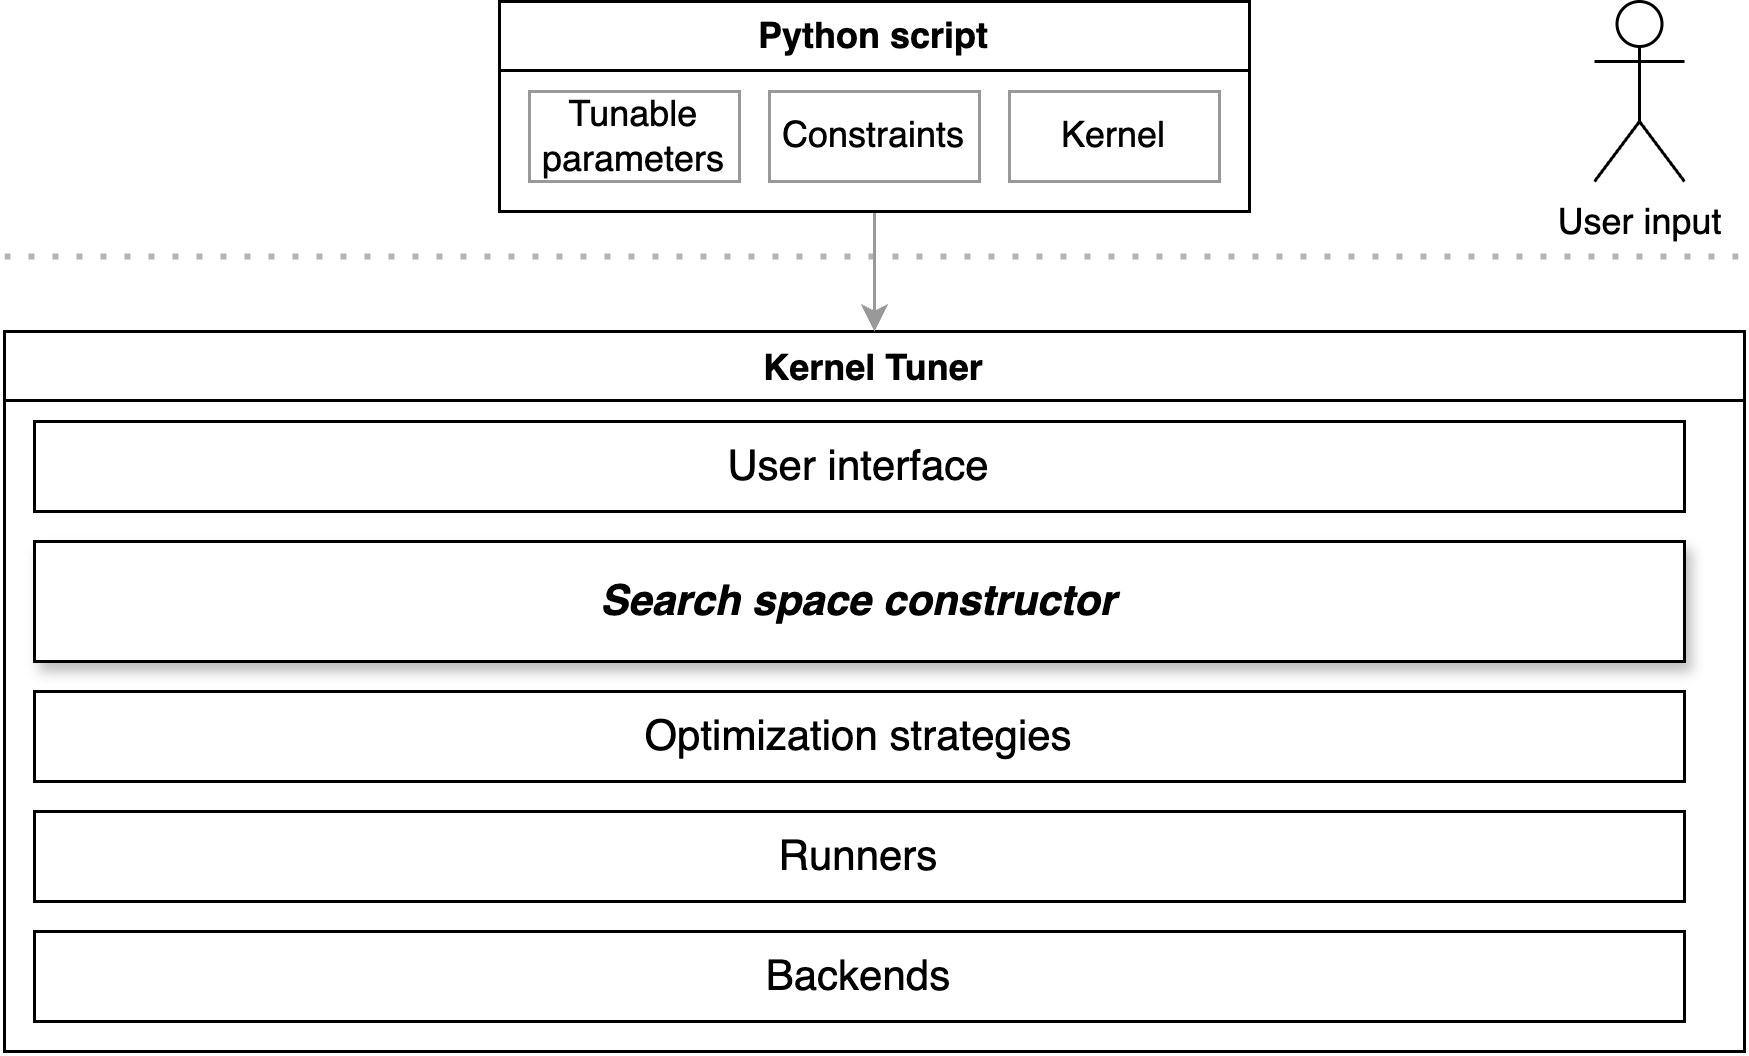
\includegraphics[width=\linewidth]{ics25template/figures/kt_architecture_simplified.png}
    \caption{Abstract Kernel Tuner software architecture.}
    \Description[Kernel Tuner software architecture]{A diagram of the Kernel Tuner software architecture, including the user inputs and external backends.}
    \label{fig:kernel-tuner-architecture}
\end{figure}

\subsection{Problem and Solution Context} \label{subsec:searchspace_construction_context}
To understand the background of the search space construction problem and explore various approaches to solutions in this subsection in an auto-tuning context, we focus on a specific auto-tuning framework.
In \cref{sec:related_work}, we discussed three open-source auto-tuning frameworks that use brute-force search space construction, which suffices for auto-tuning problems that could be manually explored, but can take a substantial amount of time with the large search spaces currently encountered. 
As in this work we aim to provide a generic efficient solution for the construction of large search spaces for auto-tuning, we implement this in the most actively developed of these three open-source auto-tuning frameworks, Kernel Tuner, to demonstrate our novel method.

Kernel Tuner is an external framework for developers to benchmark and optimize GPU kernels in isolation, which can be used with applications in any host programming language. 
The abstract software architecture of Kernel Tuner is shown in Figure~\ref{fig:kernel-tuner-architecture}. Users of Kernel Tuner create a small Python script that points to the kernel and describes both the tunable parameters and any constraints (referred to as {\em restrictions} by Kernel Tuner) to filter out invalid combinations of parameter values. 
There are also various optional settings that users can specify, such as derived metrics to be computed, the optimization objective to use, which optimization algorithm to use, and hyperparameters to the optimization algorithm of choice. 

Search space construction is the first step towards auto-tuning any function or application, preceding the search through the myriad of configurations or code variants. This is apparent from \cref{fig:kernel-tuner-architecture}, where the modular structure of Kernel Tuner is shown, with processing flowing generally from the top (user input), through the search space constructor, to the strategies (optimization algorithms) that determine the next configuration to evaluate, to the runners that prepare the evaluation, and the backends that compile and execute the kernel. After execution, the process flows back up in the diagram, either to the strategies to determine the next configuration based on the new result and repeat the process, or by reporting the best configuration found to the user. 

% In this section, we explore a fundamental change to the search space construction process, leading to a speedup of several orders of magnitude.     

% This section examines the performance improvements that have been made 
% As auto-tuning tools become more efficient, increasingly larger search spaces become feasible. As a result of this development, the efficiency with which all valid configurations (configurations that meet constraints specified by the user) are found, can have a significant impact on the total tuning time. 
% This section examines performance improvements for search space construction in Kernel Tuner. 
% This section discusses the performance improvements in Kernel Tuner for search space construction, and compares this performance to the state of the art in auto-tuning search space construction: Auto-Tuning Framework (ATF) \cite{raschATFGenericAutoTuning2017}. 

In this work, we will focus on the \textit{search space constructor} part of \cref{fig:kernel-tuner-architecture}, as with possibly billions of code variants to enumerate in a high-dimensional space, where user-defined constraints cut out parts of the space that are considered invalid, constructing the search space can become a bottleneck at the start of the tuning process. 
In GPU auto-tuning, the Cartesian product of the tunable parameters, that is, the collection of all possible combinations of all parameter values, tends to contain many configurations that are not valid. For example, because the product of the thread block sizes can not be larger than some hardware limitation, or because some combination of parameter values would lead to incorrect results in the kernel. To filter out such configurations, the user can specify constraints on certain combinations of tunable parameter values. 

The most straight-forward solution is brute force: generate all the combinations of parameter values and filter out combinations based on the user-specified constraints, leaving only valid configurations. This is reasonable for small search spaces but becomes increasingly time-consuming as the search space size and number of constraints increase.
Hence, to improve performance on large search spaces, the search space must be constructed more efficiently. 

One approach could be to resolve the constraints dynamically, either by only checking the constraints of combinations suggested by the optimization strategy before executing kernel configurations, or by resolving the search space in parallel while executing. 
However, these dynamic approaches pose problems. 
If we take the approach of only checking combinations suggested by the strategy, in tuning problems with sparse search spaces (where the vast majority of combinations of parameter values are not valid configurations), a substantial amount of time would be spent on finding any valid configuration as for each combination the optimization strategy needs to be consulted and the combination checked against the constraints. 
This problem is exacerbated by the fact that during the tuning process, the number of valid non-executed configurations decreases. To illustrate this, in the case of a random search on a search space of 100 valid configurations in a search space where 99\% is invalid (10000 combinations) and configurations are taken from the search space once executed, the expected number of attempts required to find a valid first configuration is 100. % 1/(100/10000)
However, the expected number of attempts required to find the fiftyfirst valid configuration is 199, and the sum of expected attempts required from the first to the fiftyfirst valid configuration is over 7000 - over two-thirds of the total Cartesian size of the space. % 1/(50/(10000-(-50+100))=199
While this can be mitigated by keeping track of all attempted combinations, this by itself produces a large memory footprint. 
Moreover, dynamic resolution can skew initial sampling and strategies, as the knowledge of the constraints is not fully incorporated in the search. % This can be as illustrated as follows: given a search space with two parameters, $X$ and $Y$, both with values $(2, 3, 4)$, this results in nine possible combinations of these parameter values. Adding the constraint $X > Y$ leaves three valid configurations: $((3,2),(4,2),(4,3))$. If want to take a random configuration from this search space, these three configurations ideally have an equal chance of being drawn. However, if we have previously drawn the 
% The final problem with dynamic search space resolution is particularly 

An example of a dynamic approach to search space resolution in auto-tuning is the chain-of-tree approach used by ATF~\cite{ATF} as described in \cref{subsec:related_work_software_autotuning}. While this is efficient for search spaces where the vast majority of possible combinations are invalid, individual constraints may only use a small subset of all the parameters to achieve this efficiency. 
In addition, search space characteristics such as the true parameter bounds, which can help optimization algorithms navigate the space more efficiently and enable fairly distributed sampling methods such as Latin Hypercube Sampling~\cite{willemsenBayesianOptimizationAutotuning2021}, are not resolved with the dynamic approach. Furthermore, randomized sampling is inherently biased to the sparser parts of the tree, although this has been addressed by BaCO~\cite{BaCO2024}. Moreover, selecting neighbors of configurations as extensively used by various optimization algorithms in Kernel Tuner is potentially expensive. 

Instead, we aim to fully resolve the search space before starting the tuning process, with a minimal impact on the total execution time, to incorporate the full information of the search space in the initial sampling and search strategies. 

\subsection{Using Constraint Solvers in Auto-tuning} \label{subsec:searchspace_construction_packages}
In general, this type of problem, where parameter values and constraints are resolved to valid combinations, can be encoded as a Boolean Satisfiability Problem (SAT) \cite{biereHandbookSatisfiabilityVolume2009}, Satisfiability Modulo Theories (SMT) \cite{barrett2008satisfiability}, or Constraint-Satisfaction Problem (CSP) \cite{brailsfordConstraintSatisfactionProblems1999}. At the time of writing, several frameworks are readily available as Python packages that have implemented solvers for these types of problems: \textit{CSP-solver} \cite{maniCSPSolverLibrarySolve}, \textit{Google ORTOOLS} \cite{llcOrtoolsGoogleORTools}, \textit{PicoSAT} \cite{schnellPycosatBindingsPicosat}, \textit{CPMpy} \cite{gunsCPMPy}, \textit{PyChoco} \cite{prudhommePychocoPythonBindings}, \textit{SATisPy} \cite{laszloSatispyInterfaceSAT}, \textit{PySMT} \cite{teamPySMTSolveragnosticLibrary}, \textit{python-constraint} \cite{niemeyerPythonconstraintPythonconstraintModule}. 
Nevertheless, not all of these frameworks can be applied to auto-tuning; they have their limitations in how expressive and efficient they are. In general, the SAT, SMT, and CSP problem types mentioned serve different purposes, owing to their different origins. SAT solvers are generally most efficient, at the cost of expressivity, as they are highly optimized for propositional logic problems. SMT solvers allow for non-integer finite domains such as floating-point numbers, strings, and lists, and as such are more expressive, although not as optimized as SAT solvers. CSP solvers offer high-level abstractions suitable for modeling complex constraints, providing special types such as "all-different" \cite{stojadinovicMeSATMultipleEncodings2014}, which are otherwise difficult to efficiently express, making them ideal for complex combinatorial constraints. 

In auto-tuning, the constraint problem consists of a set of named parameters, each parameter having a finite list of possible values, usually numeric but also strings or other types. As such, SMT and CSP solvers are the best fit in this case, % discarding \textit{ORTOOLS}, \textit{PicoSAT}, \textit{CPMpy}, and \textit{SATisPy} as these provide or expose SAT solvers. That leaves 
leaving \textit{CSP-solver}, \textit{PyChoco}, \textit{PySMT}, and \textit{python-constraint}. In addition, there are practical considerations when it comes to choosing a solver; \textit{PyChoco} is in beta at the time of writing and requires building from source, and \textit{PySMT} requires manual steps to install actual solvers, making it cumbersome to deploy as a dependency within a framework. Various solvers, such as \textit{CSP-solver} and the Microsoft Z3 solver in \textit{PySMT}, aim to find any solution, rather than all solutions, as required in the case of auto-tuning. To obtain all solutions, such solvers must iteratively find a solution, add this solution as an additional constraint, and look for the next solution until there are no solutions left \cite{bjornerProgrammingZ32019}. If there are many solutions, as is commonly the case with auto-tuning problems, this can have a substantial impact on performance. 

Hence, we focus on \textit{python-constraint}, as this is a CSP-based Python package with built-in support to find all solutions. Initially developed by Gustavo Niemeyer and afterwards maintained by Sébastien Celles, the \textit{python-constraint} package was first released in 2005. The more than 22000 weekly downloads\footnote{\url{https://pypistats.org/packages/python-constraint}} at the time of writing indicate that the package has a substantial user base. 

\subsection{Implementation of Optimizations} \label{subsec:searchspace_construction_improvements}
Based on \cref{subsec:searchspace_construction_packages}, we use the \textit{python-constraint} package as a basis for our implementation. To obtain the level of performance required to construct auto-tuning search spaces efficiently, we implement several key improvements in various areas: algorithmically (\cref{subsubsec:searchspace_construction_improvements_algorithm}), by extending and improving constraints (\cref{subsubsec:searchspace_construction_improvements_constraints}), by introducing parsing (\cref{subsubsec:searchspace_construction_improvements_parser}), by providing tailored output formats (\cref{subsubsec:searchspace_construction_improvements_output_formats}), and finally engineering (\cref{subsubsec:searchspace_construction_improvements_engineering}). 

\subsubsection{Algorithm} \label{subsubsec:searchspace_construction_improvements_algorithm}
We select and optimize a backtracking solver optimized for finding all solutions rather than any solution. This algorithm maintains a dictionary of variable assignments and uses a stack-based approach to implement iterative backtracking, avoiding recursive function calls. Variables are selected dynamically using a combination of the Minimum Remaining Values (MRV) and Degree heuristics, prioritizing those with fewer remaining values and higher connectivity. For each selected variable, domain values are checked against the constraints. If a constraint is violated, the algorithm backtracks by restoring previous states from a queue until all possibilities are explored. 
We have optimized this algorithm by sorting the variables on the number of internal constraints, making it faster to find unassigned variables, and by reducing the number of sorts required. 
By systematically iterating through variable assignments and leveraging heuristics, the algorithm efficiently constructs all valid solutions while minimizing unnecessary exploration. 

\subsubsection{Constraints} \label{subsubsec:searchspace_construction_improvements_constraints}
We expand and improve built-in specific constraints to optimize operations that are commonly used. 
Commonly used operations allow for increased efficiency over generic functions by applying knowledge of the operation. For example, given a constraint where $p \cdot q > 0$, we know to ignore all cases where $(p \leq 0) \xor (q \leq 0)$. 
We added \textit{MaxProduct} and \textit{MinProduct} constraints as they are commonly used in auto-tuning constraints (e.g. a maximum product of block sizes due to hardware limits). We also rewrote and added preprocessing steps to the \textit{Function}, \textit{MaxSum} and \textit{MaxProduct} constraints.  
The \textit{Function} constraint is particularly interesting for optimization, as it is both a computationally expensive constraint due to its generality and a common occurrence as it is used wherever the more specific constraints do not apply. We have optimized this by employing function rewriting and dynamic runtime compilation, as the one-off expense of compilation to bytecode is offset by the potentially many times a \textit{Function} constraint is executed. % Bytecode is a low-level representation of code specific to the Python virtual machine (PVM), which executes the bytecode to perform the desired operations.
% Given that the \textit{Function} constraint is both a common occurrence as it is used wherever the more specific constraints do not apply and a generally more computationally expensive constraint due to its generality and the fact that it may call on external functions, it has been optimized in particular by employing function rewriting and runtime compilation. 

\subsubsection{Parser} \label{subsubsec:searchspace_construction_improvements_parser}
We introduce a parser for constraints written in string format, which has three important benefits: to apply the more efficient specific constraints instead of generic functions where possible, to break down constraints into the smallest subsets of variables, thereby aiding the constraints solver, and to provide all of this without requiring users to write their constraints in a complex format that requires understanding how the solvers work. 

To address the latter benefit first, most solvers and tuners require specific function calls or a form of domain-specific language when defining the constraints (as will be encountered in \cref{subsec:evaluation_compared_frameworks}). However, as opposed to the users of CSP-solvers, auto-tuning users are generally not aware of the search space construction process and the specific constraints available that result in efficient resolution of the search space. 
Instead, we provide users the option to write their constraints in Python-evaluable string format, which is then automatically optimized by parsing. 
This usage of Python-evaluable strings has various benefits, as they are both familiar to the user as Python is already the interface language, and rewritable by our parser, allowing the application of specific constraints instead of generic functions and the decomposition of constraints into subsets. 

In particular, the automatic reduction of constraints can be important in scalability and efficiency in practice, as users unfamiliar with the intrinsics of constraint solving, such as the users of auto-tuning frameworks, might write sub-optimal constraints in practice. 
For example, consider the constraint $3 \leq X \cdot Y < 9 \leq Z$, where \textit{X}, \textit{Y}, and \textit{Z} are tunable parameters with numerical values. 
Constraints can not be evaluated until values for the involved parameters are at least partially resolved, resulting in subpar performance in the case of compound statements like the given example, as it depends on three parameters as-is. 
This can be improved by automatically breaking down the constraint into multiple constraints with fewer involved variables where possible. 
For the given example this can be [$3 \leq X \cdot Y$, $X \cdot Y < 9 $, $9 \leq Z$], which allows partially resolved values for either \textit{X}, \textit{Y}, or \textit{Z} to be enough to discard configurations not meeting the constraint earlier in the construction process. 
In addition, this automatic reduction enables the application of specific constraints, as is the case with the example, which can be represented with specific constraints as \lstinline{[(MinProd(3), [x,y]), (MaxProd(9-1), [x,y]), (MinProd(9), [z])]}. As discussed in \cref{subsubsec:searchspace_construction_improvements_constraints}, application of specific constraints can preemptively exclude values through preprocessing, resulting in an even more efficient construction. 

\subsubsection{Output Formats} \label{subsubsec:searchspace_construction_improvements_output_formats}
We implement various output formats to avoid expensive rearrangements to different formats. 
Expensive rearrangement of the structure in which solutions are output by the solver is mitigated by providing output formats that are close to the internal representation, further described in \cref{subsec:searchspace_construction_searchspace_object}.

\subsubsection{Employing C-extensions} \label{subsubsec:searchspace_construction_improvements_engineering}
In general, C and similar languages outperform Python in terms of execution speed~\cite{pythonVSC,comparingSixLanguages}. To attain this level of performance without losing the flexibility and user-friendliness of Python~\cite{pythonVSC++usability}, we employ C-extensions. 
We transpile the codebase from Python to C-code using Cython~\cite{behnelCythonBestBoth2011}, which is then compiled into Python-importable C-extensions. 
We added type hints where possible to aid in compilation. 
Binaries are precompiled for Linux, macOS, and Windows on the supported Python versions (3.9 through 3.13 as of this writing). \\

While the improvements detailed in \cref{subsubsec:searchspace_construction_improvements_algorithm,subsubsec:searchspace_construction_improvements_constraints,subsubsec:searchspace_construction_improvements_parser,subsubsec:searchspace_construction_improvements_output_formats,subsubsec:searchspace_construction_improvements_engineering} are specifically intended to obtain the level of performance required to construct auto-tuning search spaces efficiently, they are generally applicable to any CSP problem. 
Our optimizations have been approved in the main branch of \textit{python-constraint}, benefitting all users of the package and the community. 

\subsection{Search space Representation} \label{subsec:searchspace_construction_searchspace_object}
With the efficient construction of search spaces implemented in \textit{python-constraint}, we consider how this is represented and applied in auto-tuning frameworks in practice to achieve a comprehensive approach. 

As per \cref{subsec:searchspace_construction_context}, after the search space construction, the optimization algorithms use the information obtained in the construction step to select configurations.
Instances of this are obtaining the true bounds of the search space to use balanced initial sampling methods or the selection of valid neighbors that have not been evaluated yet. 
As these type of operations are commonly used in auto-tuning, it can be useful to provide an abstract representation of the search space that implements these operations, providing various views and mappings on the configurations in the search space. 

We have implemented this in Kernel Tuner as the \textit{SearchSpace} class, which takes the tunable parameters and constraints based on the the user specification, constructs the search space using \textit{python-constraint}, and provides various representations and operations on the resulting search space.  
The \textit{SearchSpace} class has multiple internal representations for varying purposes, such as hash- and index-based for efficient lookups. Externally it provides a single interface for all search space-related operations, which in contrast to the initial situation where strategies would implement these operations individually, enables reuse in a modular architecture. 
For example, the mutation step in the \textit{genetic algorithms} optimization strategy requires selecting only valid neighbors within a certain Hamming distance. This, along with other neighbor selection algorithms, is implemented in the \textit{SearchSpace} class and can be indexed before running the algorithm, improving overall performance. 

While we focus on an optimized method for search space construction in auto-tuning, resulting in a generically applicable search space constructor, considering the wider context results in a comprehensive method for search space representations and operations. 
% Various other operations commonly used by the optimization algorithms have been efficiently implemented in this \textit{SearchSpace} class, such as 

% All of these changes are evaluated in synthetic and real-world tests in \Cref{sec:evaluation}. 

% To further improve the performance of \textit{python-constraint} in general and for auto-tuning search spaces specifically, we made the following additional improvements:
% \begin{itemize}
%     \item Cythonization of the codebase. This involves transpiling from Python to C-code with Cython \cite{behnelCythonBestBoth2011}, which is then compiled to Python-importable C-extensions. We added type-hints where possible to aid compilation.
%     \item Expanded and improved built-in constraints. Commonly used operations allow for increased efficiency over generic functions by applying knowledge of the operation. For example, given a restriction where $p \cdot q > 0$, if we have a minimum product constraint specified we know to ignore all cases where $p \leq 0 \lor q \leq 0$. Hence we added \textit{MaxProduct} and \textit{MinProduct} constraints as they are commonly used in auto-tuning restrictions (e.g. a maximum product of block sizes due to hardware limits). We rewrote and added pre-processing steps to the \textit{Function}, \textit{MaxSum} and \textit{MaxProduct} constraints. 
%     \item Automatic reduction and differentiation. On the Kernel Tuner side, we added a parser from restrictions written in string format with two goals: to apply the more efficient built-in constraints instead of generic functions where possible, and to break a restriction down into the smallest subset of variables, as this aids the constraints solver. 
%     \item Improved general efficiency. Several operations were taken from the inner loops of the implemented backtracking algorithm. We added new output formats to avoid expensive rearrangements to different formats. 
% \end{itemize}
% Additionally, the reliability was improved by increasing the test coverage. We improved the maintainability by adding automated workflows for testing, building, documentation, and publishing. 
% The result of these optimizations, compared against brute-force, standard \textit{python-constraint} and the state of the art in auto-tuning search space construction is seen in \Cref{subsec:evaluation_search space}. 


% section "Evaluation":
    \section{Evaluation}\label{sec:evaluation}

In this section, we evaluate the advancements presented in \cref{sec:searchspace_construction} to determine their performance and scalability impact using a case study with various applications. 
First, we discuss how we compare against the current state-of-the-art solvers in \cref{subsec:evaluation_compared_frameworks}.
% First, we discuss the way current state-of-the-art solvers are used to compare against in \cref{subsec:evaluation_compared_frameworks}. 
Following this, we evaluate the solvers on a collection of synthetically generated search spaces to assess scalability differences between solvers under various search space characteristics in \cref{subsec:evaluation_synthetic}. 
Finally, we evaluate the solvers on a variety of real-world applications to indicate actual performance in \cref{subsec:evaluation_real-world}. 

% \Cref{sec:searchspace_construction} proposed a new approach and several optimizations to the search space construction. 
% To assess the performance of this new approach, synthetic and real-world tests are performed, to assess scaling differences under various characteristics and to indicate real-world performance, respectively. 

The evaluations in this work are performed on the sixth generation DAS \href{https://www.cs.vu.nl/das/clusters.shtml}{VU-cluster}~\cite{DASMediumScaleDistributedSystem} using an NVIDIA A4000 GPU node. The GPU is paired with a 24-core AMD EPYC-2 7402P CPU, 128 GB of memory, and running Rocky Linux 4.18. While none of the tested solvers use the GPU, we use a GPU node to obtain an environment as similar as possible to real-world GPU auto-tuning. 
For all tests performed, the results of each solver were validated against a brute-forced solution of the search space. 

% \subsection{Experimental Setup} \label{subsec:evaluation_setup}
% To assess the feasibility of tuning large search spaces with Kernel Tuner, this evaluation is performed on four applications with large search spaces. 
% The selected kernels are the top-three kernels by search space size in the Benchmark suite for Auto-Tuners (BAT) \cite{BenchmarkingSuiteKerneltuners}. These are \textit{Dedispersion}, \textit{Hotspot}, \textit{ExpDist}. In addition, we use the search space of the \textit{MicroHH} computational fluid dynamics kernel \cite{MicroHH2017}. The characteristics of these search spaces are seen in \Cref{tab:searchspaces_real_world_overview}. 

% \begin{table}[tbh]
%     \centering
%     \small
%     \begin{tabularx}{\linewidth}{|X|X|X|X|}
%         \hline
%         \textbf{Name} & \textbf{Cartesian size} & \textbf{Dimensions} & \textbf{Restrictions} \\
%         \hline
%         Dedispersion & 22272 & 8 & 3 \\\hline
%         Expdist & 9732096 & 10 & 4 \\\hline
%         Hotspot & 22200000 & 11 & 5 \\\hline
%         Microhh & 1166400 & 13 & 8 \\
%         \hline
%     \end{tabularx}
%     \caption{Overview of the characteristics of the search spaces evaluated on.}
%     \label{tab:searchspaces_real_world_overview}
% \end{table}

\subsection{Comparison against state-of-the-art} \label{subsec:evaluation_compared_frameworks}
To provide additional reference on the performance in this evaluation, we compare the results to the state-of-the-art in auto-tuning search space construction: Auto-Tuning Framework (ATF) \cite{raschATFGenericAutoTuning2017}, which specifically focuses on large optimization spaces with interdependent parameters. 
ATF has two independent implementations, in C++ and Python, both of which we use in this evaluation to compare our method to. The C++ version available as of August 2024 with Python bindings is used and denoted as \textit{ATF} in the results. The Python version, called \textit{pyATF}, is used at version 0.0.9, the latest version at the time of writing.

For the majority of the discussed solvers, the notation of tunable parameters and constraints is largely separated (e.g. a user first defines the tunable parameters and values, then defines the constraints to apply). However, both implementations of ATF have a notation that combines the definition of tunable parameters, values, and constraints into one statement. As a result of this, constraints can only reference tunable parameters that have been previously defined. Due to the large number of search spaces used in this evaluation, it is not feasible to write each of these search space definition files by hand for both ATF implementations, and we have instead written parsers that define the ATF search space files from an abstract definition of the search spaces. These parsers take the aforementioned parameter-constraint order relation into account and convert to built-in ATF types such as intervals where applicable to provide search space definitions that are as closely possible to what is expected by the authors. 
To reflect the user experience as accurately as possible, the search space file compilation time is included in the total construction time. 
The C++ version of ATF and search space files is compiled with GCC 9.4.0 using the optimization commands recommended by the ATF documentation. 

In addition, we compare against PySMT at version 0.9.6 using the Microsoft Z3 solver to evaluate differences in scalability for solvers without support for resolving all solutions, as described in \cref{subsec:searchspace_construction_packages}. The Z3 theorem prover is developed by Microsoft for software verification and analysis \cite{Z3solver}, and is the winner of the 3rd Annual Satisfiability Modulo Theories Competition (SMT-COMP)~\cite{smtcomp2007}. 
Similarly to ATF, we have written a parser to use PySMT-specific operations where applicable. 

\ifdoubleblind
We have published the implementation of this evaluation in a repository for further reference.
\else
We have published the implementation of this evaluation in a repository\footnote{\href{https://github.com/fjwillemsen/kernel_tuner_paper}} for further reference.
\fi

\subsection{Synthetic Tests} \label{subsec:evaluation_synthetic}
To understand how search space characteristics influence the construction time of the evaluated solvers, we use synthetic tests. 
We have generated a set of search spaces with a varying number of dimensions (between 2 and 5), target Cartesian sizes (with $\{1\times 10^{4}, 2\times 10^{4}, 5\times 10^{4}, 1\times 10^{5}, 2\times 10^{5}, 5\times 10^{5}, 1\times 10^{6}\}$), and number of constraints (between 1 and 6). While these arbitrary parameters result in search spaces that are not as large and do not have as many tunable parameters as the real-world search spaces evaluated on in \cref{subsec:evaluation_real-world}, the goal of these in total 112 synthetic search spaces is to gain insight into which of these factors has the greatest effect on performance, and which solution provides good scalability across the variations in these factors.
% $\{10000, 20000, 50000, 100000, 200000, 500000, 1000000\}$

\begin{figure}[!htb]
    \centering
    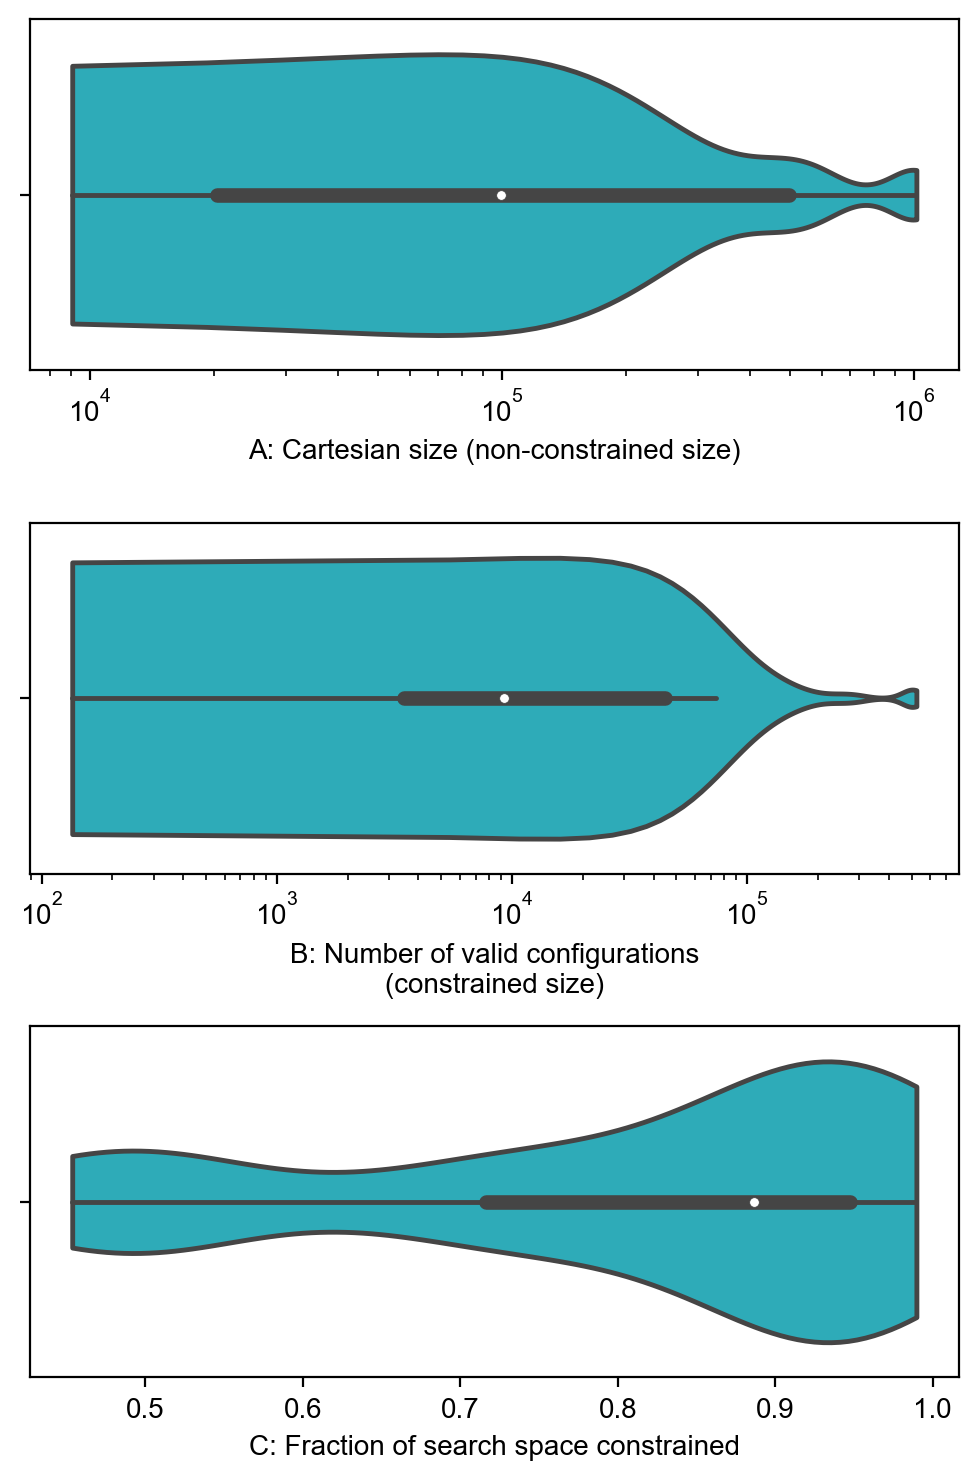
\includegraphics[width=0.95\linewidth]{ics25template/figures/searchspace_construction/results_synthetic_violin.png}
    \caption{Characteristics of the 112 synthetic search spaces}
    \Description[Characteristics of the 112 synthetic search spaces]{Characteristics of the 112 synthetic search spaces}
    \label{fig:searchspaces_synthetic_characteristics}
\end{figure}

\begin{figure*}[!htb]
    \centering
    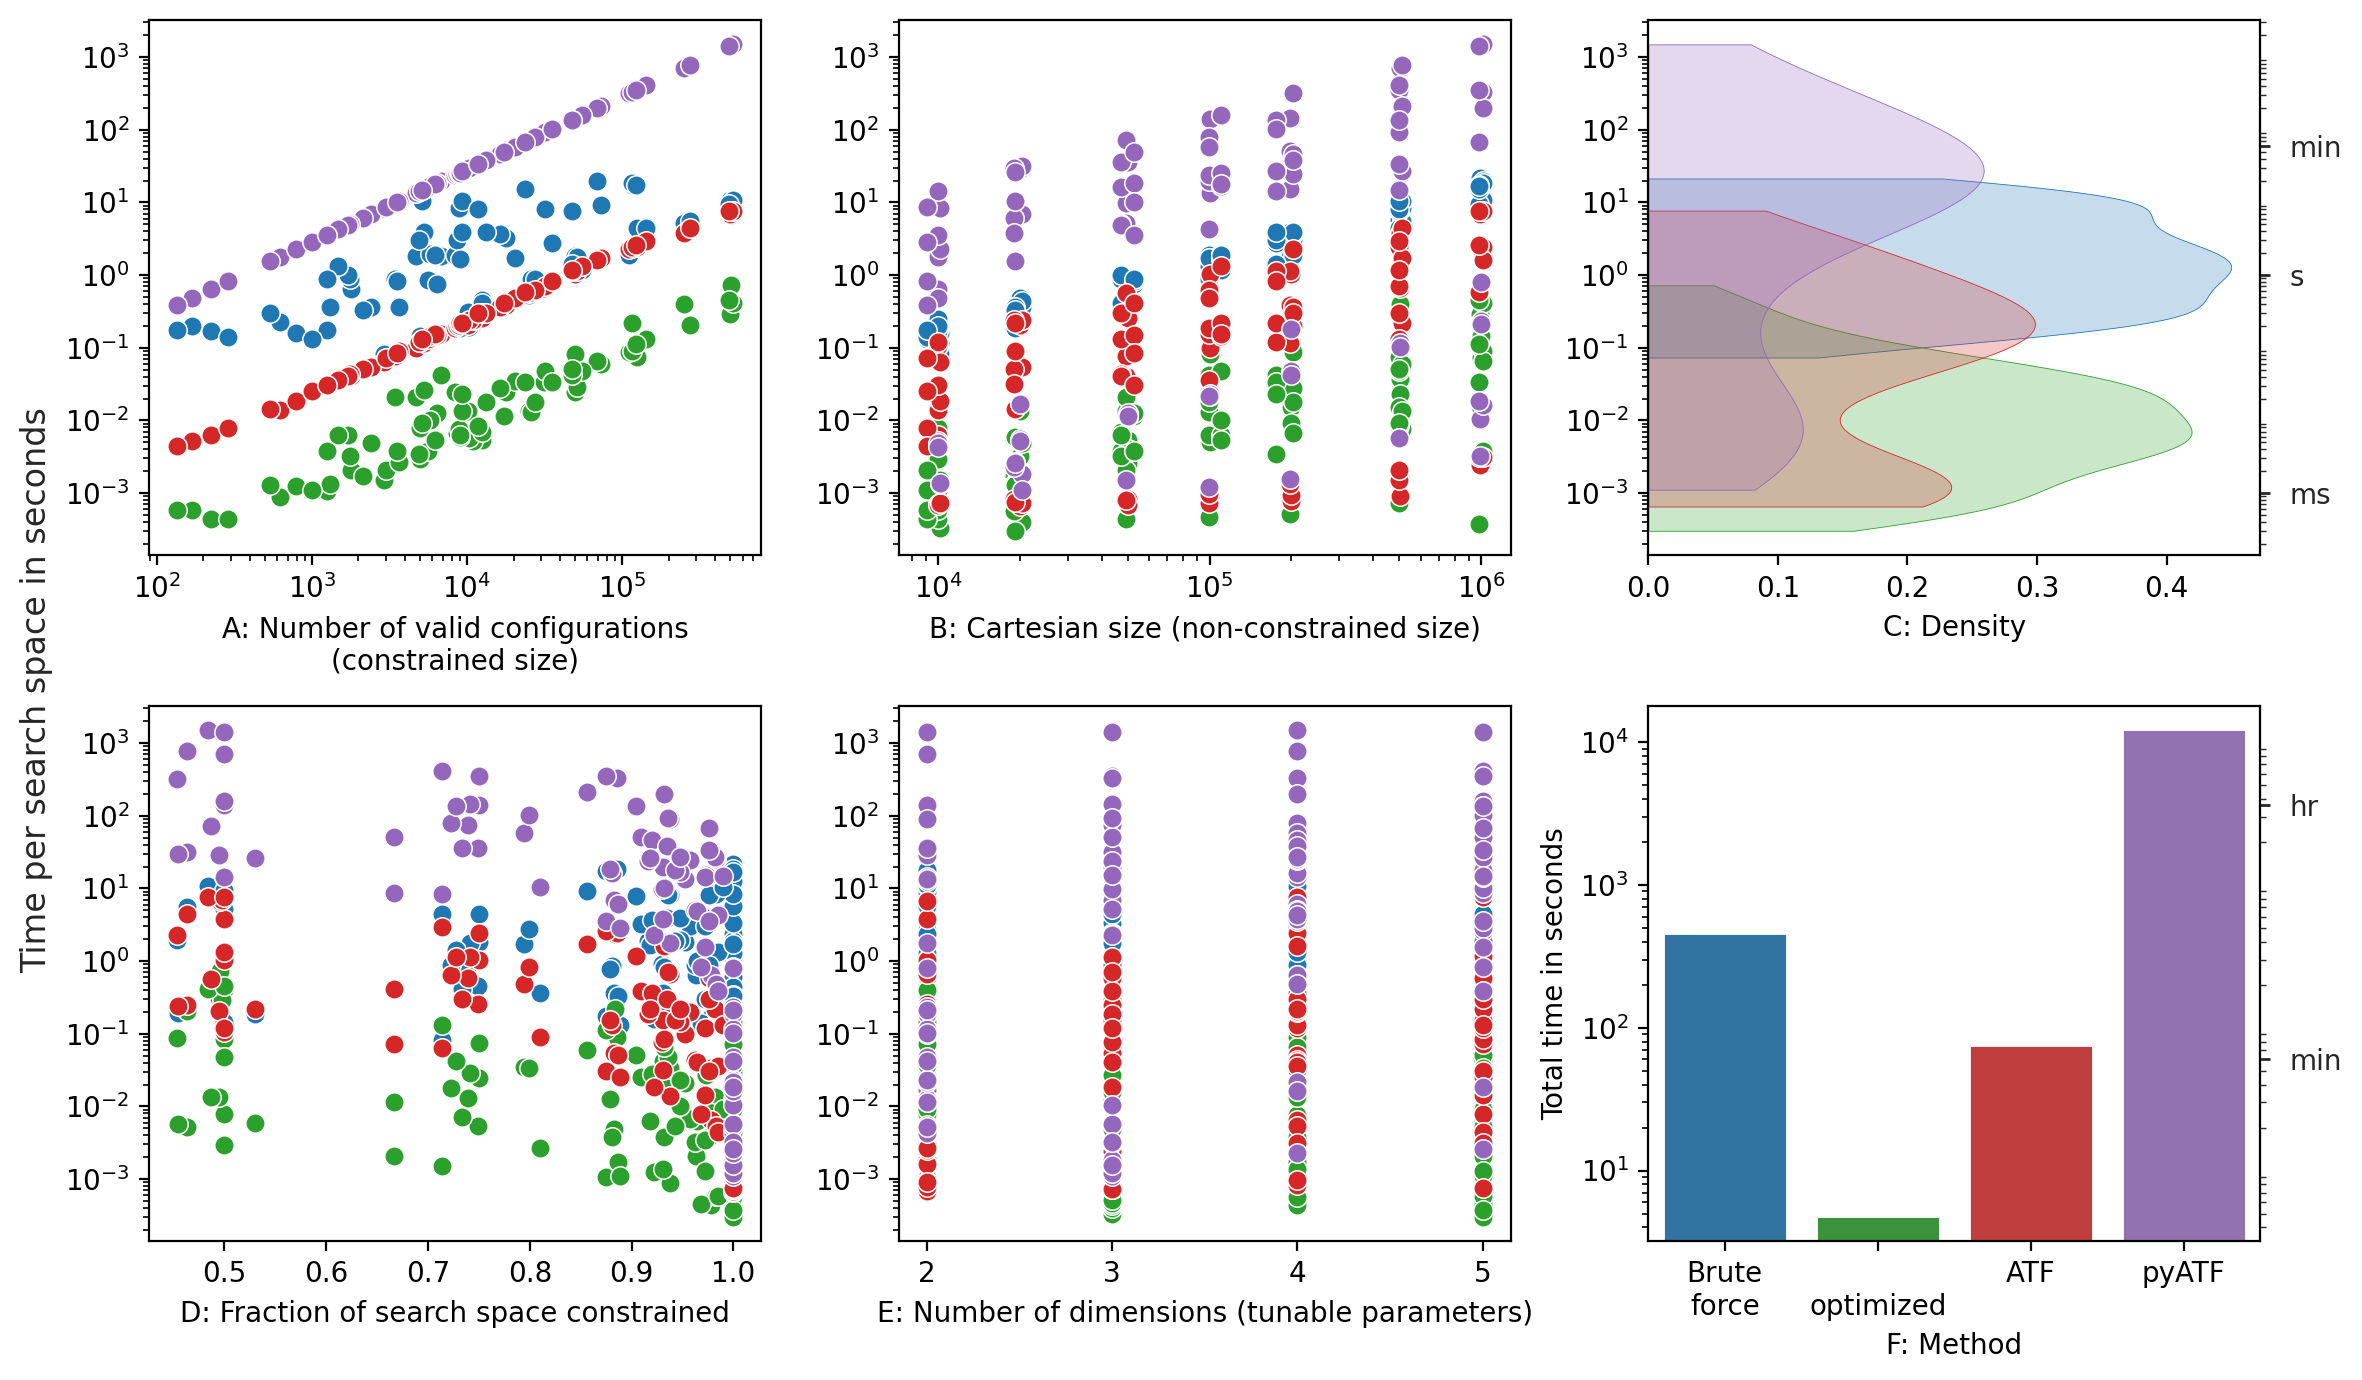
\includegraphics[width=1.0\textwidth]{ics25template/figures/searchspace_construction/results_synthetic.png}
    \caption{Search space construction performance on synthetic tests. Lower times are better. Colors correspond to \Cref{fig:results_synthetic}F barplot methods.}
    \Description[search space construction performance]{search space construction performance on synthetic tests. Lower times are better.}
    \label{fig:results_synthetic}
\end{figure*}

Given a Cartesian size, a number of dimensions, and a number of constraints, we want to generate a synthetic search space. 
To prevent an unfair advantage to solvers optimized for a limited number of dominant dimensions, this number of values per dimension $v$ is kept approximately uniform. 
This is done by first determining the number of values per dimension as $v = s^{\frac{1}{d}}$, where $s$ is the desired Cartesian size and $d$ is the desired number of dimensions. 
For each of the dimensions, a linear space with $v$ number of elements is instantiated. 
Given a non-integer value of $v$, this is rounded to an integer for all but the last dimension, where $v$ is rounded contradictory (e.g. $5.8 \rightarrow 5$, $5.2 \rightarrow 6$) to be closer to the desired Cartesian size. 
A list of constraints involving a variety of operations is generated for each combination of dimensions, which are randomly chosen up to the desired number of constraints. 

\Cref{fig:searchspaces_synthetic_characteristics} shows the dispersion of the resulting 112 search spaces in violin plots for three characteristics: the Cartesian size, the number of valid configurations, and the fraction of the search space constrained (the number of valid configurations relative to the total Cartesian size). 
As the application of the constraints does not affect the already uniformly distributed number of parameters, this characteristic is not included in the figure. 
These violin plots should be interpreted by examining both the y-axis width and central tendencies of the distributions. The wider sections indicate a higher density of search spaces with the associated x-axis values, while the white dot represents the median, and the thick bar around it marks the interquartile range.
\Cref{fig:searchspaces_synthetic_characteristics}A shows the actual Cartesian size, representing the total number of possible configurations before constraints are applied, revealed to be in line with the set of target values used. 
\Cref{fig:searchspaces_synthetic_characteristics}B depicts the number of valid configurations remaining after constraints are enforced, which follows a distribution similar to the Cartesian size of \Cref{fig:searchspaces_synthetic_characteristics}A, yet covering a wider range on the lower end, also demonstrating the general effect of constraints on the difference between the Cartesian size and actual number of configurations. 
Finally, \Cref{fig:searchspaces_synthetic_characteristics}C displays the fraction of sparsity of the search space, i.e. the fraction of non-valid configurations relative to the Cartesian size. 
Though the fraction of constrained configurations is skewed toward higher values, indicating a propensity towards sparsity, a wide range of variations in sparsity is present. 


The performance on the synthetic search spaces is displayed in various plots in \Cref{fig:results_synthetic}, where the colors used correspond to the colors of the methods in the \Cref{fig:results_synthetic}F barplot. 

It is noteworthy how in \cref{fig:results_synthetic}A there appears to be an approximately linear correlation between the time required to construct a search space and the number of valid configurations, which is not as evident in the other characteristics in \cref{fig:results_synthetic}B, \cref{fig:results_synthetic}D, and \cref{fig:results_synthetic}E. 
% Furthermore, \cref{fig:results_synthetic}A illustrates the relationship between the number of valid configurations (constrained size) and the time required to construct the search space. 
Our \textit{optimized} solver consistently achieves the lowest execution times, with several orders of magnitude better performance compared to the \textit{brute force}, \textit{ATF}, and \textit{pyATF} solvers. The \textit{pyATF} solver exhibits the highest execution times, being generally outperformed even by brute-force solving, an interesting result which we will examine using the other characteristics. 

\cref{fig:results_synthetic}B examines the effect of the Cartesian size on execution time, where a general trend of increasing computation time with larger Cartesian sizes can be seen. Interestingly, the \textit{ATF} and \textit{pyATF} solvers in some cases do not conform to this trend, creating a large variance in their performances.

The reason for this appears to be found in \cref{fig:results_synthetic}D, which shows the relationship between the fraction of the sparsity of a search space and execution time. Both \textit{ATF} and \textit{pyATF} appear to be severely optimized for very sparse search spaces, in contrast to the other methods. 

\Cref{fig:results_synthetic}C presents the execution time distributions of the solvers as a continuous probability density curve using a kernel density estimate (KDE). Particularly noteworthy is the bimodality demonstrated by \textit{ATF} and \textit{pyATF}, which appears to be caused by the sensitivity to search space sparsity seen in \cref{fig:results_synthetic}D.

Observing \cref{fig:results_synthetic}E, it appears that there is no strong correlation between solver performance and the number of tunable parameters. 

\Cref{fig:results_synthetic}F summarizes the overall performance of each solver in a bar chart.
It is remarkable that pyATF takes considerably longer than the brute-force method on these search spaces, which might be due to how optimized the ATF approach is to highly sparse search spaces.
Our optimized method achieves a 96x speedup over the brute-force method (4.75 seconds versus 455.3 seconds), a 16x speedup over ATF, and a 2547x speedup over pyATF. 
% Total speedup of method 'optimized' (4.75 seconds) over 'Bruteforce' (455.29 seconds): 95.9x
% Total speedup of method 'ATF' (74.08 seconds) over 'Bruteforce' (455.29 seconds): 6.1x
% Total speedup of method 'pyATF' (12098.64 seconds) over 'Bruteforce' (455.29 seconds): 0.0x

% The performance on the synthetic search spaces is seen in \Cref{fig:results_synthetic}, where the colors used correspond to the colors of the methods in the \Cref{fig:results_synthetic}F barplot. In \Cref{fig:results_synthetic}, it can be seen that the duration is generally more influenced by the total size of the search space (in particular the constrained size of \cref{fig:results_synthetic}A) than the ratio of valid to non-valid configurations (\cref{fig:results_synthetic}D) or the number of dimensions (\cref{fig:results_synthetic}E). \Cref{fig:results_synthetic}F shows the overall performance difference, indicating that the optimized method achieves a 96x speedup over the brute-force method (4.75 seconds versus 455.3 seconds). 
% In contrast, pyATF takes considerably longer than the brute force method on these search spaces. % Both pyATF and ATF appear to scale linearly with the number of valid configurations. 
% It is noteworthy that the C++ version of ATF comes somewhat close to the performance of our optimized method, but only when nearly all of the search space is constrained, as seen in \cref{fig:results_synthetic}D. 
% Both the ATF and pyATF density distributions interestingly demonstrate bimodality in the top plot of \cref{fig:results_synthetic}C, which intersects with the performance difference of both implementations over the fraction of search space constrained in \cref{fig:results_synthetic}D, confirming that the ATF approach is heavily optimized for very sparse search spaces.
% In general, our new method is $\sim$96x faster than brute force, $\sim$15x faster than ATF, and $\sim$2547x faster than pyATF on these synthetic search spaces. 
% % Synthetic: 
% % Total speedup of method 'Old' (675.44 seconds) over 'Bruteforce' (455.29 seconds): 0.7x
% % Total speedup of method 'New' (4.75 seconds) over 'Bruteforce' (455.29 seconds): 95.9x
% % Total speedup of method 'ATF' (74.08 seconds) over 'Bruteforce' (455.29 seconds): 6.1x
% % Total speedup of method 'pyATF' (12098.64 seconds) over 'Bruteforce' (455.29 seconds): 0.0x
% % Real-world: 
% % Total speedup of method 'Old' (8347.66 seconds) over 'Bruteforce' (65197.71 seconds): 7.8x
% % Total speedup of method 'New' (2.88 seconds) over 'Bruteforce' (65197.71 seconds): 22668.4x
% % Total speedup of method 'ATF' (135.3 seconds) over 'Bruteforce' (65197.71 seconds): 481.9x
% % Total speedup of method 'pyATF' (2474.65 seconds) over 'Bruteforce' (65197.71 seconds): 26.3x

\begin{figure}[!htb]
    \centering
    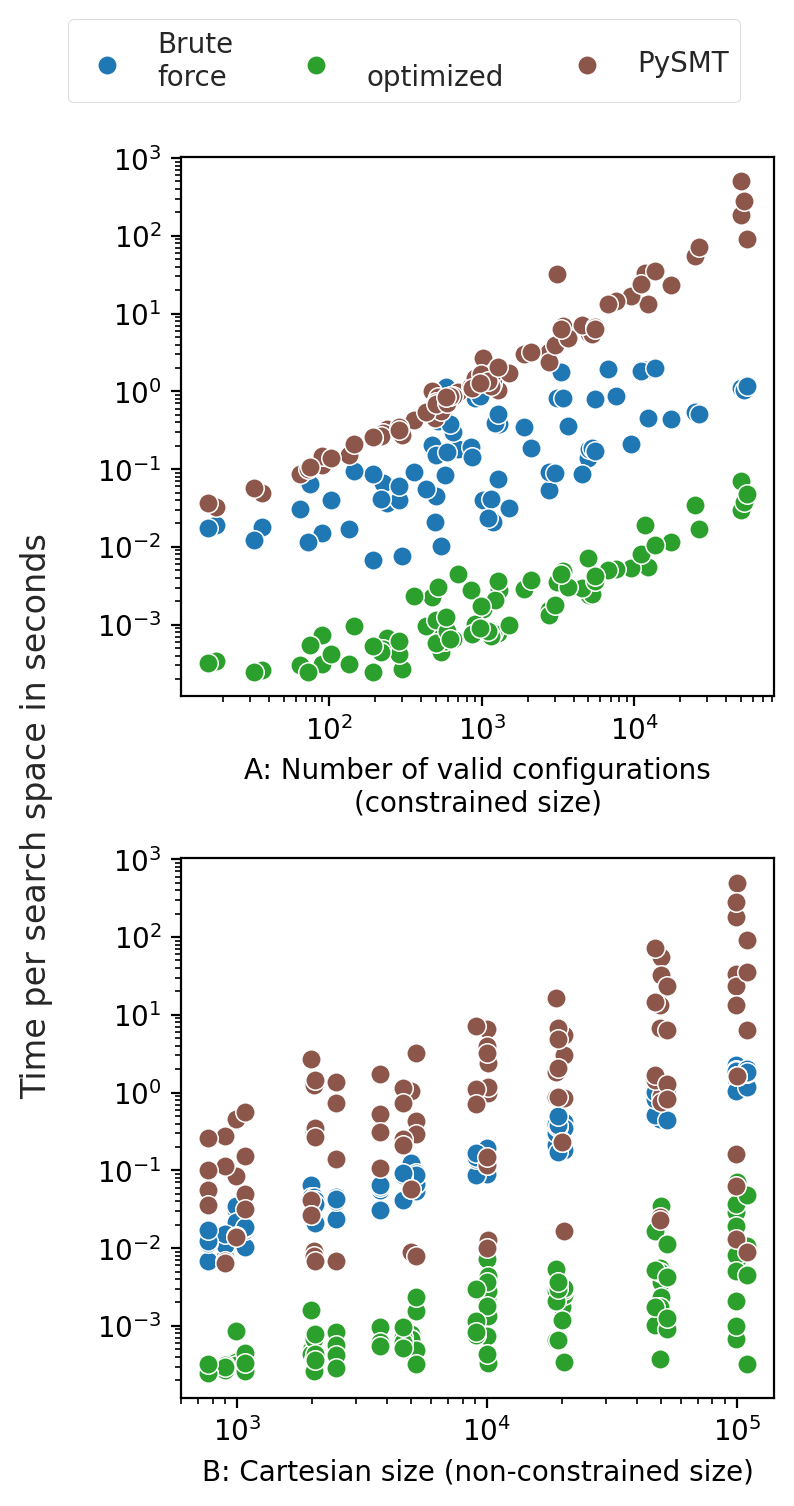
\includegraphics[width=0.95\linewidth]{ics25template/figures/searchspace_construction/results_synthetic_pysmt_100000.png}
    \caption{Search space construction performance of PySMT on synthetic tests (reduced search spaces size).}
    \Description[search space construction performance synthetic with PySMT]{search space construction performance on synthetic tests, including PySMT.}
    \label{fig:results_synthetic_pysmt}
\end{figure}

As described in \cref{subsec:searchspace_construction_packages}, a traditional solver without support for finding all solutions requires adding the previous solution as a constraint and iterating over the solutions until all solutions have been found. To demonstrate the lack of scalability of such a solver, \cref{fig:results_synthetic_pysmt} compares PySMT using the Microsoft Z3 solver to the brute-force method and the optimized solver. 
To make executing this experiment feasible, we had to reduce the size of the generated synthetic search spaces by one order of magnitude in this instance. 
As seen in \cref{fig:results_synthetic_pysmt}, PySMT performs poorly relative to both brute force and our optimized method. As expected, this difference increases as the number of valid configurations increases, demonstrating the infeasibility of this approach when many valid configurations are present. 
Despite the reduced search space sizes, PySMT with the Z3 solver still takes nearly a thousand seconds on the largest search spaces, whereas the brute-force solver takes about ten seconds. 
Our optimized solver takes about as long to solve the largest search spaces as PySMT with the Z3 solver takes to solve the smallest search spaces. PySMT with the Z3 solver will not be included in the remainder of the evaluation as it is infeasible to evaluate the large search spaces of the real-world applications. 

% Total speedup of method 'original' (8353.17 seconds) over 'Brute
% force' (65230.47 seconds): 7.8x
% Total speedup of method '
% optimized' (3.16 seconds) over 'Brute
% force' (65230.47 seconds): 20610.7x
% Total speedup of method 'ATF' (137.83 seconds) over 'Brute
% force' (65230.47 seconds): 473.3x
% Total speedup of method 'pyATF' (2816.74 seconds) over 'Brute
% force' (65230.47 seconds): 23.2x

% old results:
% Total speedup of method 'Old' (6.79 seconds) over 'Bruteforce' (4.55 seconds): 0.7x
% Total speedup of method 'New' (0.07 seconds) over 'Bruteforce' (4.55 seconds): 63.8x
% Total speedup of method 'ATF' (1.07 seconds) over 'Bruteforce' (4.55 seconds): 4.3x
% Total speedup of method 'pyATF' (121.72 seconds) over 'Bruteforce' (4.55 seconds): 0.0x
% Total speedup of method 'PySMT' (88.25 seconds) over 'Bruteforce' (4.55 seconds): 0.1x


\subsection{Real-world Applications} \label{subsec:evaluation_real-world}

\begin{table*}[htb]
    \centering
    \scriptsize
    \begin{tabularx}{\linewidth}{|l|X|X|X|X|X|X|X|X|}
        \hline
        % \textbf{Name} & \textbf{Cartesian size} & \textbf{Constraint size} & \textbf{Number of parameters (dimensions)} & \textbf{Number of constraints} & \textbf{Avg. unique parameters per constraints} & \textbf{Range of number of values per parameter} & \textbf{\% of configurations in Cartesian size}  \\
        % \hline
        % Dedispersion & 22272 & 11130    & 8 & 3     & 2 & 1 - 29 & 49.973 \\\hline
        % ExpDist & 9732096 & 294000      & 10 & 4    & 2 & 1 - 11 & 3.021 \\\hline
        % Hotspot & 22200000 & 349853     & 11 & 5    & 3.8 & 1 - 37 & 1.576 \\\hline
        % GEMM & 663552 & 116928          & 17 & 8    & 3.25 & 1 - 4 & 17.622 \\\hline
        % MicroHH & 1166400 & 138600      & 13 & 8    & 2.375 & 1 - 10 & 11.883 \\\hline
        % ATF PRL 2x2 & 36864 & 1200      & 20 & 14   & 2.429 & 1 - 3 & 3.255 \\\hline
        % ATF PRL 4x4 & 9437184 & 10800   & 20 & 14   & 2.429 & 1 - 4 & 0.114 \\\hline
        % ATF PRL 8x8 & 2415919104 & 48720 & 20 & 14  & 2.429 & 1 - 8 & 0.002 \\\hline
        % \textit{Mean} & \textit{307322534} & \textit{121403} & \textit{14.875} & \textit{8.75}  & \textit{2.589} & \textit{1} - \textit{13.25} & \textit{10.93} \\\hline
        
        \textbf{Name} & \textbf{Cartesian size} & \textbf{Constraint size} & \textbf{Number of parameters (dimensions)} & \textbf{Number of constraints} & \textbf{Avg. unique parameters per constraints} & \textbf{Range of number of values per parameter} & \textbf{\% of configurations in Cartesian size} & \textbf{Avg. number of constraint evaluations required}  \\
        \hline
        Dedispersion & 22272 & 11130    & 8 & 3     & 2 & 1 - 29 & 49.973     & 33414 \\\hline
        ExpDist & 9732096 & 294000      & 10 & 4    & 2 & 1 - 11 & 3.021      & 23889240 \\\hline
        Hotspot & 22200000 & 349853     & 11 & 5    & 3.8 & 1 - 37 & 1.576    & 65900294 \\\hline
        GEMM & 663552 & 116928          & 17 & 8    & 3.25 & 1 - 4 & 17.622   & 2576736 \\\hline
        MicroHH & 1166400 & 138600      & 13 & 8    & 2.375 & 1 - 10 & 11.883 & 4763700 \\\hline
        ATF PRL 2x2 & 36864 & 1200      & 20 & 14   & 2.429 & 1 - 3 & 3.255   & 268680 \\\hline
        ATF PRL 4x4 & 9437184 & 10800   & 20 & 14   & 2.429 & 1 - 4 & 0.114   & 70708680 \\\hline
        ATF PRL 8x8 & 2415919104 & 48720 & 20 & 14  & 2.429 & 1 - 8 & 0.002   & 18119076600 \\\hline
        \hline
        \textit{Mean} & \textit{307322534} & \textit{121403} & \textit{14.875} & \textit{8.75}  & \textit{2.589} & \textit{1} - \textit{13.25} & \textit{10.93} & \textit{2285902168} \\\hline
    \end{tabularx}
    \caption{Overview of the basic characteristics of the real-world search spaces and the mean values for each of the columns.}
    \label{tab:searchspaces_real_world_overview}
\end{table*}
% Avg. unique involved parameters per restriction:
% d = [[2,2,2], [2,2,2,2], [2,2,2,6,7], [2,3,3,3,3,4,4,4], [4,3,2,2,2,2,2,2], [2,2,2,2,3,3,3,2,2,2,3,3,3,2]]    # last entry is the same for all PRL spaces
% for s in d:
%   print(round(sum(s)/len(s), 3))

To evaluate solver performance on the search spaces of real-world applications, we select the three largest search spaces in the Benchmark suite for Auto-Tuners (BAT)~\cite{BenchmarkingSuiteKerneltuners}. 
These are \textit{Dedispersion}, \textit{Hotspot}, and \textit{ExpDist}. 
In addition, we use the relatively large search spaces of the commonly used General Matrix Multiplication kernel \textit{(GEMM)}~\cite{CLBlast2018} and \textit{MicroHH} computational fluid dynamics kernel~\cite{MicroHH2017}. 
To provide a fair comparison to ATF, the Probabilistic Record Linkage (\textit{PRL}) kernel used by the ATF paper~\cite{searchspaceATF} is used as well, resulting in three additional search spaces for a total of eight real-world search spaces. 
The characteristics of the real-world search spaces are displayed in \cref{tab:searchspaces_real_world_overview}, where the rightmost column denotes the average number of constraint evaluations that are required to brute-force solve a search space. For each combination in the Cartesian product, all constraints need to be evaluated until the combination is rejected or all constraints have been evaluated. Hence the average number of constraint evaluations can be calculated by taking the average of the best case (the first constraint rejects the combination) and worst case (the last constraint rejects the combination), and adding all valid combinations which are never rejected. Given a search space $S$, let $S_i$ be the set of non-valid combinations, $S_v$ the set of valid combinations, and $S_c$ the set of constraints, the average number of constraint evaluations can be calculated as $\frac{|S_i|+|S_i| \cdot |S_c|}{2}+|S_v|$. 
Descriptions of each of the kernels and their search spaces are given in \cref{subsubsec:evaluation_setup_kernel_dedispersion,subsubsec:evaluation_setup_kernel_expdist,subsubsec:evaluation_setup_kernel_hotspot,subsubsec:evaluation_setup_kernel_gemm,subsubsec:evaluation_setup_kernel_microhh,subsubsec:evaluation_setup_kernel_atf_prl}, before the results are discussed in \cref{subsubsec:evaluation_real-world_results}.

\subsubsection{Dedispersion} \label{subsubsec:evaluation_setup_kernel_dedispersion}
\iflackofspace
The Dedispersion kernel presented in \cite{BenchmarkingSuiteKerneltuners} is designed to compensate for the time delay experienced by radio waves as they propagate through space. This delay occurs due to the frequency-dependent dispersion of the signal. By applying a specific dispersion measure (DM) and reversing the dispersion effect, the kernel reconstructs the original signal.
During the iteration over frequency channels, threads process multiple time samples and dispersion measures in parallel.
\else
The Dedispersion kernel presented in \cite{BenchmarkingSuiteKerneltuners} is designed to compensate for the time delay experienced by radio waves as they propagate through space. This delay occurs due to the frequency-dependent dispersion of the signal. By applying a specific dispersion measure (DM) and reversing the dispersion effect, the kernel reconstructs the original signal. In this context, the signal at the highest frequency \(f_{h}\) arrives at time \(t_{x}\), whereas lower frequencies emitted simultaneously arrive at \(t_{x} + k\), where \(k\) represents the delay in seconds and is calculated using the following equation:
\begin{equation}
k \approx 4150 \times DM \times \left( \frac{1}{f_{i}^2} - \frac{1}{f_{h}^2} \right)
\end{equation}
The kernel takes as input time-domain samples across multiple frequency channels and produces dedispersed samples for a range of DM values. During the iteration over frequency channels, threads process multiple time samples and dispersion measures in parallel.
\fi
Comparing the Dedispersion search space to the other real-world search spaces tested on in \cref{tab:searchspaces_real_world_overview}, the resulting search space is the smallest in Cartesian size, but as it has the highest percentage of valid configurations at nearly 50~\%, it is not the smallest in number of valid configurations. 

% % Original:
% The Dedispersion kernel in \cite{BenchmarkingSuiteKerneltuners} aims to mitigate the time delay caused by the propagation of radio waves through space. This process involves applying a specific dispersion measure and reverse-dispersing the signal to recover its original form. The signal with the highest frequency \(f_{h}\) arrives at time \(t_{x}\), while the lower frequencies emitted at the same time arrive at time \(t_{x} + k\), where \(k\) is the delay in seconds according to the following equation:
% \begin{equation}
%     k \approx 4150 \times DM \times ( \frac{1}{f_{i}^2} \times \frac{1}{f_{h}^2} )
% \end{equation}
% The kernel inputs samples in time across many frequency bands, and outputs dedispersed samples corresponding to a range of dispersion measure (DM) values. While iterating over the frequency channels, the threads can work on multiple samples and dispersion measurements in parallel. 
% Comparing the Dedispersion search space to the other real-world search spaces tested on in \cref{tab:searchspaces_real_world_overview}, the resulting search space is the smallest in Cartesian size, but as it has the highest percentage of valid configurations, it is not the smallest in number of valid configurations. 
% % Because the kernel is inherently memory bound~\cite{sclocco2014}, the performance assessment is conducted in terms of GB/s:\begin{equation}    \frac{nr\_dms \times nr\_samples \times nr\_channels}{\textit{time}}\end{equation}where \(nr\_dms = 2048\) is the number of dispersion measures, \(nr\_samples = 25000\) is the number of time samples, and \(nr\_channels = 1536\) is the number of frequency channels. These settings correspond to the configuration used by the APERTIF telescope~\cite{sclocco2020amber}.In Table \ref{DedispTable}, we can see an overview of all the tunable parameters used by the Kernel Tuner tuning runs. With these parameters, we obtain a total of 22272 different configurations before applying restrictions. 

% From BAT paper:
% The Dedispersion kernel in BAT originates from the AMBER pipeline for the detection of single pulse astronomical transients~\cite{sclocco2020amber}.
% Dedispersion is the process of reverting the dispersion of a radio signal transmitted over many frequencies through space. 
% The signal component with the highest frequency $f_h$ is received at time $t_x$, while simultaneously emitted components with lower frequency arrive at $t_x + k$, where $k$ is the delay in seconds as by the dispersion equation:
% \begin{equation*}
%     k \approx 4150 \times DM \times \left( \frac{1}{f_i^2} \times \frac{1}{f_h^2} \right)
% \end{equation*}

% The kernel takes samples in time across many frequency bands (channels) as input and outputs the dedispersed samples for many different dispersion measure $DM$ values. The kernel is parallelized such that each thread can work on multiple samples and dispersion measures while iterating over the frequency bands. As input for the BAT Dedispersion kernel, we are using the parameters from the ARTS survey on the Apertif telescope~\cite{van2022apertif}, which uses a sampling rate of 24.4 KHz, 2048 DMs, and 1536 channels.

% The tunable parameters of the dedispersion kernel are shown in Table~\ref{tab:dedisp-parameters}. 
% The \verb|loop_unroll_factor_channel| parameter depends on the input, as any divisor of the number of channels can be used as a partial loop unrolling factor for the inner loop in the kernel. When the loop unroll factor is 0, it is left to the CUDA compiler to decide whether or not to apply loop unrolling. \verb|tile_stride_x| controls the stride used to vary the amount of work per thread. When \verb|tile_stride_x| is 0 and \verb|tile_size_x| is larger than 1, threads will process \verb|tile_size_x| consecutive samples when \verb|tile_stride_x| is 1 thread will process \verb|tile_size_x| samples that are each \verb|block_size_x| apart in the input. \verb|tile_stride_y| works similarly but for dispersion measures in the y-dimension.
% \begin{table}[ht]
%     \caption{Tunable parameters -- Dedispersion kernel in BAT.}
%     \centering
%     \begin{tabular}{l|p{3cm}|l}
%     \toprule
%     Parameter & Values & \# \\
%     \midrule
% \verb|block_size_y| & $\{1,2,4,8,16n \mid 16n \in [16, 512] \}$ & 36 \\
% %\verb|block_size_x|  & \{1, 2, 4, 8, 16, 32, 48, 64, 80, 96, 112, 128, 144, 160, 176, 192, 208, 224, 240, 256, 272, 288, 304, 320, 336, 352, 368, 384, 400, 416, 432, 448, 464, 480, 496, 512\} & 36 \\
% \verb|block_size_y|  & $\{4n \mid 4n \in [4,128]\}$ & 32 \\
% %\{4, 8, 12, 16, 20, 24, 28, 32, 36, 40, 44, 48, 52, 56, 60, 64, 68, 72, 76, 80, 84, 88, 92, 96, 100, 104, 108, 112, 116, 120, 124, 128\} & 32 \\
% %\verb|tile_size_x|  & \{1, 2, 3, 4, 5, 6, 7, 8, 9, 10, 11, 12, 13, 14, 15, 16\} & 16 \\
% %\verb|tile_size_y|  & \{1, 2, 3, 4, 5, 6, 7, 8, 9, 10, 11, 12, 13, 14, 15, 16\} & 16 \\
% \verb|tile_size_x|  & $\{ n | n \in [1, 16] \}$ & 16 \\
% \verb|tile_size_y|  & $\{ n | n \in [1, 16] \}$ & 16 \\
% \verb|tile_stride_x|  & \{0, 1\} & 2 \\
% \verb|tile_stride_y|  & \{0, 1\} & 2 \\
% \verb|loop_unroll_factor_channel|  & \{0, 1, 2, 3, 4, 6, 8, 12, 16, 24, 32, 48, 64, 96, 128, 192, 256, 384, 512, 768, 1536\} & 21 \\
% \verb|blocks_per_sm|  & \{0, 1, 2, 3, 4\} & 5 \\
%     \bottomrule
%     \end{tabular}
% %    \caption{Tunable parameters -- Dedispersion kernel in BAT.}
%     \label{tab:dedisp-parameters}
% \end{table}

\subsubsection{ExpDist} \label{subsubsec:evaluation_setup_kernel_expdist}
\iflackofspace
The ExpDist kernel described in~\cite{BenchmarkingSuiteKerneltuners} is utilized in a localization microscopy application that performs template-free particle fusion by integrating multiple observations into a single super-resolution reconstruction~\cite{heydarian2018template}. During the registration process, the ExpDist kernel is repeatedly invoked to evaluate the alignment of two particles.
The algorithm exhibits quadratic complexity with respect to the number of localizations per particle, making it highly computationally intensive. 
\else
The ExpDist kernel described in~\cite{BenchmarkingSuiteKerneltuners} is utilized in a localization microscopy application that performs template-free particle fusion by integrating multiple observations into a single super-resolution reconstruction~\cite{heydarian2018template}. During the registration process, the ExpDist kernel is repeatedly invoked to evaluate the alignment of two particles. The distance between particles $t$ and $m$, given a registration $M$, is calculated as follows:
\begin{equation}
    D = \sum\limits_{i=1}^{K_t} \sum\limits_{j=1}^{K_m} \textrm{exp}\left( - \frac{\|\vec{x}_{t,i} - M(\vec{x}_{m,j})\|^2 }{ 2\sigma^2} \right)
\end{equation}
The kernel operates directly on the individual localizations ($\vec{x_t}$ and $\vec{x_m}$) in each particle rather than pixelated images, accounting for uncertainties in the localizations ($\sigma$). The algorithm exhibits quadratic complexity with respect to the number of localizations per particle, making it highly computationally intensive. 
\fi
The resulting search space is the second-most sparse of the real-world search spaces in \cref{tab:searchspaces_real_world_overview}.

% % Original
% The ExpDist kernel of~\cite{BenchmarkingSuiteKerneltuners} is part of a localization microscopy application that implements a template-free particle fusion algorithm by combining many different observations into a single super-resolution reconstruction~\cite{heydarian2018template}. The ExpDist kernel is used as part of the registration process where the kernel is called repeatedly to quantify the registration of two particles. The distance between two particles $t$ and $m$, given registration $M$, is computed as follows:
% \begin{equation}
%     D = \sum\limits_{i=1}^{K_t} \sum\limits_{j=1}^{K_m} \textrm{exp}\left( - \frac{\|\vec{x}_{t,i} - M(\vec{x}_{m,j})\|^2 }{ 2\sigma^2} \right)
% \end{equation}
% The kernel operates directly on the individual localizations ($\vec{x_t}$ and $\vec{x_m}$) in each particle rather than pixelated images and takes the uncertainties in the localizations ($\sigma$) into account. The algorithm is quadratic in the number of localizations per particle and is as such highly compute-intensive.
% % The tunable parameters used in the ExpDist kernel are shown in Table~\ref{tab:expdist-parameters}.
% % The kernel supports two main implementations that are controlled by the \verb|use_column| parameter. When \verb|use_column| is set to 1, the kernel reduces the number of thread blocks used to perform the computation by using a fixed number of thread blocks in the y dimension, set by \verb|n_y_blocks|. \verb|use_shared_mem| use shared memory selects the way in which shared memory is used.
% % \begin{table}[ht]
% %     \caption{Tunable parameters -- ExpDist kernel in BAT.}
% %     \centering
% %     \begin{tabular}{l|p{3cm}|l}
% %     \toprule
% %     Parameter & Values & \# \\
% %     \midrule
% % \verb|block_size_x| & \{32, 64, 128, 256, 512, 1024\} & 6 \\
% % \verb|block_size_y| & \{1, 2, 4, 8, 16, 32\} & 6 \\
% % \verb|tile_size_x| & \{1, 2, 3, 4, 5, 6, 7, 8\} & 8 \\
% % \verb|tile_size_y| & \{1, 2, 3, 4, 5, 6, 7, 8\} & 8 \\
% % \verb|use_shared_mem| & \{0, 1, 2\} & 3 \\
% % \verb|loop_unroll_factor_x| & \{1, 2, 3, 4, 5, 6, 7, 8\} & 8 \\
% % \verb|loop_unroll_factor_y| & \{1, 2, 3, 4, 5, 6, 7, 8\} & 8 \\
% % \verb|use_column| & \{0, 1\} & 2\\
% % \verb|n_y_blocks| & \{1, 2, 4, 8, 16, 32, 64, 128, 256, 512, 1024\} & 11 \\
% %  \bottomrule
% %     \end{tabular}
% %     \label{tab:expdist-parameters}
% % \end{table}

\subsubsection{Hotspot} \label{subsubsec:evaluation_setup_kernel_hotspot}
The Hotspot kernel in \cite{BenchmarkingSuiteKerneltuners} is part of a thermal simulation application used for estimating the temperature of a processor by considering its architecture and simulating power currents. Through an iterative process, the kernel solves a set of differential equations. The inputs to the kernel consist of power and initial temperature values, while the output is a grid displaying average temperature values across the entire chip. 
It is interesting to note that the Hotspot search space is the largest in number of valid configurations, second-largest in Cartesian size, and has the highest number of values for a single parameter. 
% The performance is assessed in GFLOP/s:\begin{equation}    \frac{\textit{temporal\_tiling\_factor} \times 15 \times 4096 \times 4096}{\textit{time}}\end{equation}Table \ref{HSTable} lists the different tunable parameters and their possible values used in the experiment runs. Without considering the restrictions applied during tuning, we have a total of 4.44 million configurations.

% From BAT paper:
% The Hotspot kernel included in BAT is based on the Hotspot kernel in the Rodinia Benchmark suite~\cite{che_rodinia_2009}. 
% The %Hotspot 
% kernel is part of a thermal simulation application used to estimate processor temperature based on processor architecture
% and simulated power currents. The kernel iteratively solves a series of differential equations. The kernel inputs are the power and initial temperatures, the output is a grid of average temperature values spanning the chip.

% % *** reorder  We have re-implemented the Hotspot kernel in Rodinia from scratch to simplify the indexing scheme and increase the tunability of the kernel. 
% To simplify the indexing scheme and increase the tunability of the kernel, we have re-implemented the Hotspot kernel in Rodinia from scratch. 
% The main difference between our implementation with that of Rodinia is that our kernel can be used with any thread block dimension, can arbitrarily vary the amount of work per thread, and vary the extent to which temporal tiling is applied.

% The tunable parameters for the Hotspot kernel in BAT are shown in Table~\ref{tab:hotspot-parameters}. 
% \verb|block_size_x| and \verb|block_size_y| describe the thread block dimensions in x and y, the kernel uses at least 32 and at most 1024 threads.
% \verb|tile_size_x| and \verb|tile_size_y| control the number of output elements computed by each thread in the x and y dimensions. \verb|temporal_tiling_factor| is the number of iterations of the stencil operation performed by a single kernel launch, for more details on the temporal tiling optimization see Hijma et al.~\cite{hijma2022}. \verb|sh_power| enables or disables the use of shared memory as a cache for storing the input power currents. \verb|blocks_per_sm| is used in the \verb|__launch__bounds()| directive in CUDA to hint the compiler to aim for a certain occupancy when running the kernel, effectively this optimization encourages the compiler to decrease register usage in the kernel.

% \begin{table}[ht]
%     \caption{Tunable parameters -- Hotspot kernel in BAT.}
%     \centering
%     \begin{tabular}{l|p{3cm}|l}
%     \toprule
%     Parameter & Values & \# \\
%     \midrule
% \verb|block_size_x| & $\{1,2,4,8,32n \mid 32n \in [32, 1024] \}$ & 37 \\
% %\verb|block_size_x| & $\{$1, 2, 4, 8, 16, 32, 64, 96, 128, 160, 192, 224, 256, 288, 320, 352, 384, 416, 448, 480, 512, 544, 576, 608, 640, 672, 704, 736, 768, 800, 832, 864, 896, 928, 960, 992, 1024$\}$ & 37 \\
% \verb|block_size_y| & $\{$1, 2, 4, 8, 16, 32$\}$ & 6 \\
% \verb|tile_size_x| & $\{$n $\mid$ n $\in$ [1, 10] $\}$& 10 \\
% \verb|tile_size_y| & $\{$n $\mid$ n $\in$ [1, 10] $\}$& 10 \\
% %\verb|tile_size_x| & $\{$1, 2, 3, 4, 5, 6, 7, 8, 9, 10$\}$ & 10 \\
% %\verb|tile_size_y| & $\{$1, 2, 3, 4, 5, 6, 7, 8, 9, 10$\}$ & 10 \\
% \verb|temporal_tiling_factor| & $\{$n $\mid$ n $\in$ [1, 10] $\}$& 10 \\
% \verb|loop_unroll_factor_t| & $\{$n $\mid$ n $\in$ [1, 10] $\}$& 10 \\
% \verb|sh_power| & $\{$0, 1$\}$ & 2 \\
% \verb|blocks_per_sm| & $\{$0, 1, 2, 3, 4$\}$ & 5 \\
%  \bottomrule
%     \end{tabular}
%     \label{tab:hotspot-parameters}
% \end{table}

\subsubsection{GEMM} \label{subsubsec:evaluation_setup_kernel_gemm}
Generalized dense matrix-matrix multiplication is a fundamental operation in the BLAS linear algebra library and is widely used across various application domains. GEMM is known for its high performance on GPU hardware and has frequently served as a benchmark in studies of GPU code optimization~\cite{CLTune,li2009note,pruning}.
In this evaluation, we utilize the GEMM kernel from CLBlast~\cite{CLBlast2018}, a tunable OpenCL BLAS library. 
\iflackofspace
GEMM is implemented as the multiplication of two matrices ($A$ and $B$); $C = \alpha A \cdot B + \beta C$, where $\alpha$ and $\beta$ are constants, and $C$ is the output matrix. 
\else
GEMM is implemented as the multiplication of two matrices, $A$ and $B$:
\begin{equation}
    \nonumber C = \alpha A \cdot B + \beta C
\end{equation}
where $\alpha$ and $\beta$ are constants, and $C$ is the output matrix. 
\fi
The dimensions of all three matrices are set to $2048 \times 2048$, resulting in a relatively dense search space.

% Original:
% Generalized dense matrix-matrix multiplication (GEMM) is part of the BLAS linear algebra library and is one of the most widely used kernels across many application domains. GEMM is well known to perform very efficiently on GPU hardware and has been the example kernel in many studies of GPU code optimization~\cite{CLTune,li2009note,pruning}.
% In this evaluation, we use the GEMM kernel implemented in CLBlast~\cite{CLBlast2018}, a tunable OpenCL BLAS library. GEMM is implemented as the multiplication of two matrices, $A$ and $B$:
% \begin{equation}
%     \nonumber C = \alpha A \cdot B + \beta C
% \end{equation}
% where $\alpha$ and $\beta$ are constants and $C$ is the output matrix. We use randomly generated input data and matrix sizes of $2048 \times 2048$ for all three matrices. 
% %The performance is reported in GFLOP/s, which is computed as\begin{equation}\nonumber(2 \times N \times M \times K + N \times M + M \times K) / t\end{equation}where $N$, $M$, and $K$ are the dimensions of the matrices, and $t$ is the execution time of the kernel.The CLBlast GEMM kernel can be tuned with many parameters, here we summarize the most important ones:\begin{itemize}\item $M\sb{wg}$, $N\sb{wg}$, and $K\sb{wg}$ represent the total size of the tile processed by a single thread block in theM, N, and K matrix dimensions.\item $M\sb{dimC}$ and $N\sb{dimC}$ are the thread block dimensions in M and N.\item $M\sb{dimA}$ and $N\sb{dimB}$ can be used to control shared memory usage.%, when shared memory is used. \item $M\sb{vec}$ and $N\sb{vec}$ are the vector widths for loading and storing to global memory, $M\sb{vec}$ is used for matrices A and C, and $N\sb{vec}$ for matrix B.\item $K\sb{wi}$ is the unrolling factor used for the loop over K.\end{itemize}%Together these tunable parameters describe a very large space of which many portions are restricted as well. In total, the search space consists of 5788 legal kernel configurations, that will all be compiled and benchmarked when using the brute force strategy. 

% % From BAT paper:
% % Generalized dense matrix-matrix multiplication (GEMM) is part of the BLAS linear algebra specification, and is one of the most widely-used GPU kernels. 
% % The GEMM kernel included in BAT is from CLBlast~\cite{clblast}, a tunable OpenCL BLAS library.
% % GEMM implements the multiplication of two matrices, $A$ and $B$:
% % \begin{equation}\nonumber
% % C = \alpha A \cdot B + \beta C
% % \end{equation}
% % %
% % where $\alpha$ and $\beta$ are scalars and $C$ is the output matrix. 
% % The CLBlast GEMM kernel is tunable with the parameters shown in Table~\ref{tab:gemm-parameters}.  \verb|MWG| and \verb|NWG| control the amount of work assigned to each thread block. \verb|MDIMC| and  \verb|NDIMC| describe the size of thread block, while \verb|MDIMA| and \verb|MDIMB| control shared memory usage, \verb|VWM| and \verb|VWN| are the vector widths used for loading from and storing to global memory, and \verb|SA| and \verb|SB| enables or disables the use of shared memory for elements in $A$ and $B$.

% % \begin{table}[ht]
% %     \caption{Tunable parameters -- GEMM kernel in BAT.}
% %     \centering
% %     \begin{tabular}{l|l|l}
% %     \toprule
% %     Parameter & Values & \# \\
% %     \midrule
% %  \verb|MWG|  & $\{$16, 32, 64, 128$\}$ & 4 \\
% %  \verb|NWG|  & $\{$16, 32, 64, 128$\}$ & 4 \\
% %  \verb|MDIMC|  & $\{$8, 16, 32$\}$ & 3 \\
% %  \verb|NDIMC|  & $\{$8, 16, 32$\}$ & 3 \\
% %  \verb|MDIMA|  & $\{$8, 16, 32$\}$ & 3 \\
% %  \verb|NDIMB|  & $\{$8, 16, 32$\}$ & 3 \\
% %  \verb|VWM|  & $\{$1, 2, 4, 8$\}$ & 4 \\
% %  \verb|VWN|  & $\{$1, 2, 4, 8$\}$ & 4 \\
% %  \verb|SA|  & $\{$0, 1$\}$ & 2 \\
% %  \verb|SB|  & $\{$0, 1$\}$ & 2 \\
% %  \bottomrule
% %     \end{tabular}
% %     \label{tab:gemm-parameters}
% % \end{table}

\subsubsection{MicroHH} \label{subsubsec:evaluation_setup_kernel_microhh}
The computational fluid dynamics kernel of~\cite{MicroHH2017} is used for weather and climate modeling, specifically for the simulation of turbulent flows in the atmospheric boundary layer. 
In this case, we use the search space resulting from the auto-tunable GPU implementation of the \textit{advec\_u} kernel with extended parameter values as specified in the source of~\cite{heldensKernelLauncherLibrary2023}. % ~\footnote{\url{https://github.com/stijnh/microhh/blob/991c2d2407042edc0e3301d23137f85d0a291c98/kernel_tuner/helpers.py\#L116-L144}}
Looking at \cref{tab:searchspaces_real_world_overview}, it is notable that the MicroHH search space is the closest to the mean values of all search spaces in the number of parameters, number of constraints, and percentage of configurations. It is also second-closest in constraint size and number of values per parameter, making it perhaps the most average search space in our set of tests.

\subsubsection{ATF PRL} \label{subsubsec:evaluation_setup_kernel_atf_prl}
The Probabilistic Record Linkage (PRL) kernel used in \cite{searchspaceATF} is a parallelized implementation of an algorithm that is commonly used in data mining to identify data records referring to the same real-world entity. 
In this kernel, the input sizes determine the size of the search space. As shown in \cref{tab:searchspaces_real_world_overview}, the brute-force resolution of this search space with input sizes $8x8$ requires $1.8119 \times 10^{10}$ constraint evaluations on average, which took $\sim$27 hours to execute. % (C+CN)/2 = e (2415919104+2415919104*14)/2
As an input size of $16x16$ would require $4.639 \times 10^{12}$ constraint evaluations on average, it is not feasible to brute force beyond the $8x8$ input size. % C = 2*2*1*3*3*1*i*i*2*i*i*1*i*i*2*i*i; (618475290624+618475290624*14)/2 (the |S_v| is unkown here but due to extremely high sparsity not really relevant)
Because the brute-forced solution is used for validation and serves as a reference point in the performance comparisons, we use the search spaces resulting from the ATF PRL kernel with input sizes $2x2$, $4x4$, and $8x8$. It is notable that while the $8x8$ search space results in the largest Cartesian size of the set, the ATF PRL search spaces are very sparse. 

% We now discuss the results of the synthetic and real-world tests performed and validated against a reference solution of the search space as described in \cref{subsec:evaluation_setup} to assess the performance of the various approaches.

% For the real-world tests, we have used the largest search spaces in the Benchmark suite for Auto-Tuners (BAT) \cite{BenchmarkingSuiteKerneltuners}. These are \textit{Dedispersion}, \textit{Hotspot}, \textit{ExpDist}. In addition, we use the search space of the \textit{MicroHH} computational fluid dynamics kernel \cite{MicroHH2017}. The characteristics of these search spaces are seen in \Cref{tab:search spaces_real_world_overview}. 

% \begin{table}[tbh]
%     \centering
%     \scriptsize
%     \begin{tabularx}{\linewidth}{|X|X|X|X|}
%         \hline
%         \textbf{Name} & \textbf{Cartesian size} & \textbf{Dimensions} & \textbf{Restrictions} \\
%         \hline
%         Dedispersion & 22272 & 8 & 3 \\\hline
%         Expdist & 9732096 & 10 & 4 \\\hline
%         Hotspot & 22200000 & 11 & 5 \\\hline
%         Microhh & 1166400 & 13 & 8 \\
%         \hline
%     \end{tabularx}
%     \caption{Overview of the basic characteristics of the real-world search spaces.}
%     \label{tab:search spaces_real_world_overview}
% \end{table}

\begin{figure*}[!htb]
    \centering
    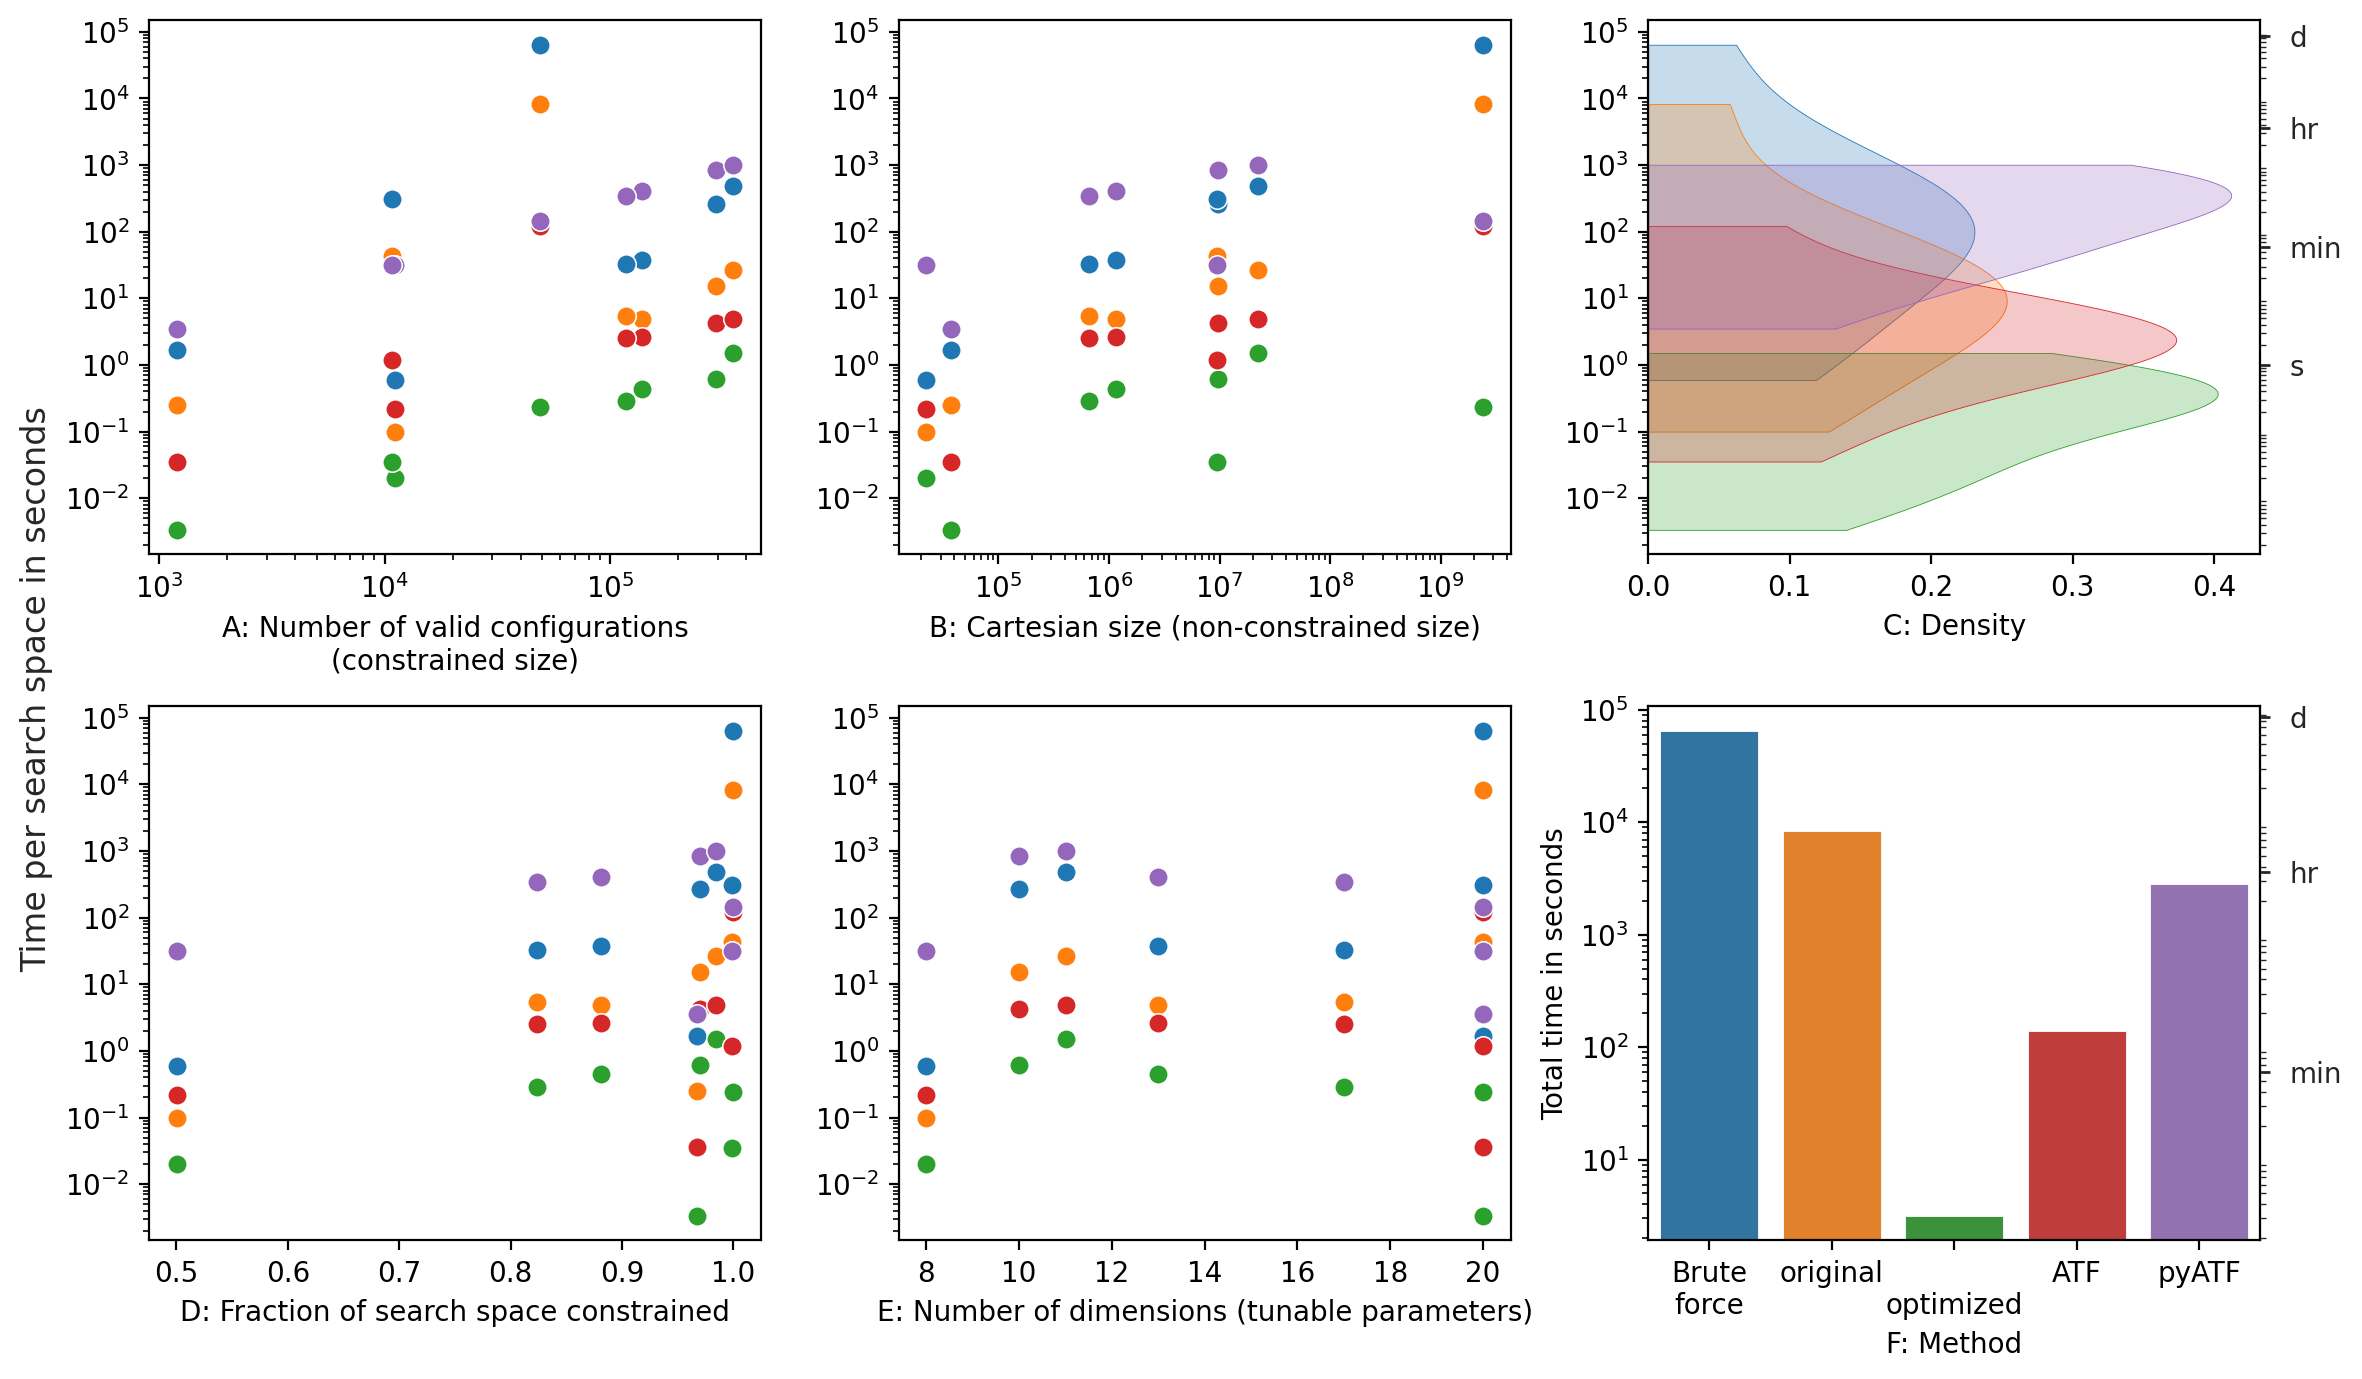
\includegraphics[width=1.0\textwidth]{ics25template/figures/searchspace_construction/results_realworld.png}
    \caption{Search space construction performance on real-world tests. Lower times are better. Colors correspond to \Cref{fig:results_realworld}F barplot methods.}
    \Description[Real-world search space construction performance]{Search space construction performance on real-world tests. Lower times are better.}
    \label{fig:results_realworld}
\end{figure*}

\subsubsection{Results} \label{subsubsec:evaluation_real-world_results}
\Cref{fig:results_realworld} presents the search space construction performance across the eight real-world benchmarks for five different constraint solver methods: \textit{brute force}, \textit{original}, \textit{optimized}, \textit{ATF}, and \textit{pyATF}. 
To determine the impact of the optimizations described in \cref{subsec:searchspace_construction_improvements}, the \textit{original} method denotes the use of vanilla \textit{python-constraint} before the optimizations, whereas our \textit{optimized} method includes the optimizations of \cref{subsec:searchspace_construction_improvements} as before in \cref{subsec:evaluation_synthetic}. 

\Cref{fig:results_realworld}A and \cref{fig:results_realworld}B illustrate the relationship between search space size and solver performance. In general, larger constrained search spaces (A) and Cartesian sizes (B) result in increased search times, particularly for the brute-force method. Our optimized solver consistently achieves the lowest execution times across all problem sizes, demonstrating its efficiency. ATF and pyATF show a similar trend but with higher execution times compared to our optimized solver, particularly for larger spaces. The original solver exhibits significantly higher execution times than our optimized version, though it performs better than the brute-force method.

\Cref{fig:results_realworld}C visualizes the distribution of execution times, providing an indication of the average performance and variability. 
Due to the substantially lower number of real-world search spaces compared to the synthetic search spaces, some observations made for \cref{fig:results_synthetic}C are obscured in \cref{fig:results_realworld}C, in particular the bimodality of the pyATF and ATF distributions. 
Nevertheless, it is interesting to observe that while the \textit{original} python-constraint method is one order of magnitude faster than the \textit{brute-force} method, both methods have very similar distributions. 
A clear trend emerges from this plot, where our optimized solver has the best performance and the least variability. 

In \cref{fig:results_realworld}D, the relation between how constrained a search space is and solver performance is displayed. 
In contrast to the synthetic tests in \cref{subsec:evaluation_synthetic}, the correlation between solver performance and the sparsity of the search space is not as clear. 
Nevertheless, \textit{ATF} and \textit{pyATF} performance again appears influenced by the sparsity, as for fraction $> 0.9$ \textit{ATF} performance is better than the \textit{original} solver, in contrast to $\leq 0.9$, where at fraction $\simeq 0.5$ even the unoptimized \textit{original} python-constraint outperforms \textit{ATF}. 

Similar to what is observed in \cref{subsec:evaluation_synthetic}, the number of tunable parameters displayed in \cref{fig:results_realworld}E do not appear to have as much of an impact on performance as the other plots discussed. 
Nevertheless, \cref{fig:results_realworld}E is useful to discern the individual search spaces based on the number of parameters. 
For instance, it can be noted that the performance difference between our optimized method and all other methods appears to be relatively stable, even for the ATF PRL search spaces detailed in \cref{tab:searchspaces_real_world_overview}, as can be discerned by the number of tunable parameters, where the three ATF search spaces have 20 tunable parameters.

Finally, \cref{fig:results_realworld}F summarizes the total time taken by each solver. 
The brute-force approach is the least performant, taking almost a full day to resolve the eight search spaces. 
Although the \textit{original} python-constraint solver is faster than brute force, our \textit{optimized} solver achieves a $\sim$2643x speedup over it, demonstrating the efficiency of our optimizations.
While ATF and pyATF achieve intermediate performance levels, the optimized solver considerably outperforms all others: our optimized method achieves a $\sim$20611x overall speedup over the brute-force method (3.16 seconds versus 65230.47 seconds), $\sim$44x over ATF, and $\sim$891x over pyATF. 
% As established in \cref{subsec:evaluation_synthetic}, these results confirm that solver performance is strongly influenced by the characteristics of the search space. 

Overall, it is noteworthy that our optimized solver consistently outperforms any alternative on all of the search spaces by a wide margin. 
These findings emphasize the advantages of our optimized solver in efficiently handling large and complex search spaces.

% Total speedup of method 'original' (8353.17 seconds) over 'Bruteforce' (65230.47 seconds): 7.8x
% Total speedup of method 'optimized' (3.16 seconds) over 'Bruteforce' (65230.47 seconds): 20610.7x
% Total speedup of method 'ATF' (137.83 seconds) over 'Bruteforce' (65230.47 seconds): 473.3x
% Total speedup of method 'pyATF' (2816.74 seconds) over 'Bruteforce' (65230.47 seconds): 23.2x


% Looking at the results of these tests in \cref{fig:results_realworld}, the performance difference is even more pronounced than in the synthetic tests: the optimized method achieves a $\sim$20611x overall speedup over the brute-force method (3.16 seconds versus 65230.47 seconds), is $\sim$44x faster than ATF, and $\sim$891x faster than pyATF. 
% It is interesting to note that the performance difference between our optimized method and all other methods appears to be relatively stable, even for the ATF PRL search spaces detailed in \cref{tab:searchspaces_real_world_overview}, as can be discerned by the number of tunable parameters in \cref{fig:results_realworld}E, where all ATF search spaces have 20 tunable parameters where the others do not.
% % On average over these real-world search spaces, our optimized method is three orders of magnitude faster than brute-forcing and one order of magnitude faster than the state-of-the-art in search space construction. 

% Finally, it is of interest to determine the impact of the optimizations. 
% In the results in \cref{fig:results_realworld}, the "\textit{original}" method denotes the use of \textit{python-constraint} before the optimizations described in \cref{subsec:searchspace_construction_improvements}, whereas the "\textit{optimized}" method includes the optimizations of \cref{subsec:searchspace_construction_improvements}. 
% While the \textit{original} method consistently outperforms \textit{bruteforce}, it does not outperform ATF and does not outperform PyATF on the ATF PRL search spaces. This is in contrast to the optimized method which consistently outperforms all other methods by a wide margin, confirming the efficacy of the optimizations. 
% % Total speedup of method 'Old' (8347.66 seconds) over 'Bruteforce' (65197.71 seconds): 7.8x
% % Total speedup of method 'New' (2.88 seconds) over 'Bruteforce' (65197.71 seconds): 22668.4x
% % Total speedup of method 'ATF' (135.3 seconds) over 'Bruteforce' (65197.71 seconds): 481.9x
% % Total speedup of method 'pyATF' (2474.65 seconds) over 'Bruteforce' (65197.71 seconds): 26.3x

% section "Conclusion"
    \section{Conclusions}
\label{sec:conclusion_futurework}

We introduced a novel approach to constructing auto-tuning search spaces for GPU kernels using an optimized Constraint Satisfaction Problem (CSP) solver, addressing the specific challenges posed by the complexity of auto-tuning and large search spaces. 
Our contributions, available to the CSP-solving and auto-tuning community in the open-source \href{https://pypi.org/project/python-constraint2/}{python-constraint} and \href{https://pypi.org/project/kernel-tuner/}{Kernel Tuner} packages, substantially outperform state-of-the-art methods in search space construction performance, enabling the exploration of previously unattainable problem scales in auto-tuning and related domains.

Through rigorous evaluation, we demonstrated that our optimized CSP-based approach reduces construction time by several orders of magnitude, even for search spaces with billions of possible combinations. 
On average over the evaluated real-world applications, our optimized method is four orders of magnitude faster than brute force, three orders of magnitude faster than the unoptimized CSP solver, and one to two orders of magnitude faster than the state-of-the-art in search space construction. 
Our optimized search space construction method reduces the construction time of real-world applications to sub-second levels, eliminating it as a substantial factor in the overall tuning process overhead. %, confirming the efficiency of this new approach to search space construction. 
This breakthrough allows researchers and developers to more effectively harness the performance potential of modern GPUs and provides an efficient generic solver for similar problem domains.

\textbf{Availability}: The methods presented in this work are available as user-friendly software packages, enabling straightforward adoption by the auto-tuning community and related fields. 
They can be installed with \lstinline{pip install python-constraint2} and \lstinline{pip install kernel-tuner}. 
Both python-constraint and Kernel Tuner are open-source software welcoming contributions. 
For more information, visit the \href{https://github.com/KernelTuner/kernel_tuner}{Kernel Tuner}\footnote{\url{https://github.com/KernelTuner/kernel_tuner}} and \href{https://github.com/python-constraint/python-constraint}{python-constraint}\footnote{\url{https://github.com/python-constraint/python-constraint}} repositories. 

\ifdoubleblind
\else
\textbf{Acknowledgments}: The CORTEX project has received funding from the Dutch Research Council (NWO) in the framework of the NWA-ORC Call (file number NWA.1160.18.316).
\fi


% Bibliography
\bibliographystyle{ACM-Reference-Format}
\bibliography{references}

\end{document}
\endinput
%%
%% End of file `sample-sigconf.tex'.